\documentclass[defaultstyle,10pt,master,Helvetica]{definitions/thesis}
% Helvetica is a similar font to Arial, with small differences.

%% Packages
\typeout{}
\typeout{--------------------------------------------------------------}
\typeout{ +---+ Thesis Template                            }
\typeout{ +---+      Version 2.0, August 2011                         }
\typeout{ +---+  for Instituto Superior Tecnico (IST),                 }
\typeout{ +---+  Universidade Técnica de Lisboa                         }
\typeout{ * Using Thesis Style form Pedro Tomás                                }
\typeout{ * Created to write Dissertations                             }
\typeout{ * Conforms with IST Master Degree format and with most important packages setup        }
\typeout{ * Should conform with IST PhD Degree format (not verified)   }
\typeout{                                                              }
\typeout{ AUTHOR: Miguel Amador and João Marques                                          }
\typeout{                                                              }
\typeout{Important: Use all files in the archive, since this is based in all them. Modify dummy files at wish.                                                              }
\typeout{--------------------------------------------------------------}
\typeout{}

% Defines an additional alphabet... not required in most cases
% ------------------------------------------------------------
% \DeclareMathAlphabet{\mathpzc}{OT1}{pzc}{m}{it}

% PACKAGE babel:
% ---------------
% The 'babel' package may correct some hyphenisation issues of latex.
% However in most situations it is not required.
\usepackage[english]{babel}

% PACKAGE fontenc:
% -----------------
% chooses T1-fonts and allows correct automatic hyphenation.
%\usepackage[T1]{fontenc}
\usepackage[latin1]{inputenc}

% Package ulem.
\usepackage{ulem} % Allows the use of other text emphatizer commands
\normalem %defines \emph{} to italic, instead of underline.
\raggedbottom %declaration makes all pages the height of the text on that page. No extra vertical space is added. The \flushbottom declaration makes all text pages the same height, adding extra vertical space when necessary to fill out the page.

% PACKAGE date time:
% -----------------
% Lets you alter the format of the date that \today returns.
\usepackage{datetime}
\newdateformat{todaythesis}{\monthname[\THEMONTH]  \THEYEAR}

% PACKAGE latexsym:
% -----------------
% Defines additional latex symbols. May be required for thesis with many math symbols.
\usepackage{latexsym}

% PACKAGE amsmath, amsthm, amssymb, amsfonts:
% -------------------------------------------
% This package is typically required. Among many other things it adds the possibility
% to put symbols in bold by using \boldsymbol (not \mathbf); defines additional
% fonts and symbols; adds the \eqref command for citing equations. I prefer the style
% "(x.xx)" for referering to an equation than to use "equation x.xx".
\usepackage{amsmath, amsthm, amssymb, amsfonts, amsbsy}

% PACKAGE multirow, colortbl, longtable:
% ---------------------------------------
% These packages are most usefull for advanced tables. The first allows to join rows
% throuhg the command \multirow which works similarly with the command \multicolumn
% The second package allows to color the table (both foreground and background)
% The third package is only required when tables extend beyond the length of one page;
% with compatibilities with the tabular environment. The last allow the definitions of landscape pages, allowing the use of a different orientation for wider graphics or tables. See package documentation to see the implementation.
\usepackage{multirow}
\usepackage{colortbl}
\usepackage{supertabular}
\usepackage{pdflscape}
% \usepackage{longtable}

% PACKAGE graphics, epsfig, subfigure, caption:
% ---------------------------------------------
% Packages for figures... well you will certainly need these packages, with the exception
% of the 'caption' package. This only allows to define extra caption options.
% Notice that subfigure allows to place figures within figures with its own caption. It
% should be avoided to create an eps file with subfigures. That will mean that you won't be
% able to reference those subfigures. Instead create an EPS file (the only graphics format supported
% by latex) for each of the subfigures and then use the command \subfigure (see below).
\usepackage{graphics}
\usepackage{graphicx}
\usepackage[caption=false]{subfig}
%\usepackage[footnotesize,bf,center]{caption}
\usepackage{dcolumn}
\usepackage{bm}
\usepackage{booktabs}
\usepackage{rotating}
\usepackage{multirow}

%\usepackage[font=small,labelfont=bf,textfont=normalfont]{caption}

% PACKAGE algorithmic, algorithm
% ------------------------------
% These packages are required if you need to describe an algorithm.
% \usepackage{algorithmic}
% \usepackage[chapter]{algorithm}

% PACKAGE natbib/cite
% -------------------
% The two packages are not compatible, and you should use one of the two. Notice however that the
% IEEE BiBTeX stylesheet is imcompatible with the natbib package. If using the IEEE format, use the
% cite package instead
\usepackage[square,numbers,sort&compress]{natbib}
%\usepackage{cite}

% PACKAGE acronyum
% -----------------
% This package is most useful for acronyms. The package guarantees that all acronyms definitions are
% given at the first usage. IMPORTANT: do not use acronyms in titles/captions; otherwise the definition
% will appear on the table of contents.
\usepackage[printonlyused]{acronym}
\usepackage[titletoc,title,header]{appendix}
\usepackage[noauto]{chappg}

% PACKAGE extra_functions VER COMO DEVE SER
% -----------------
% My Personal package: defines the following commands:
% \fancychapter{chaptername) -> Prints a fancier chapter (you can also use the fancychapter package for this)
% \hline{width} -> use for a replacement of the \hline command
% \Mark1, \Mark2, \Mark3, ...
\usepackage{definitions/extra_functions}


% PACKAGE hyperref
% -----------------
% Set links for references and citations in document
% Some MiKTeX distributions have faulty PDF creators in which case this package will not work correctly
% Long live Linux :D
\usepackage[plainpages=false]{hyperref}
\hypersetup{
  colorlinks=false,
  citecolor=none,
  linkcolor=none,
  breaklinks=true,
  bookmarksnumbered=true,
  bookmarksopen=true,
  pdftitle={Memristors-based recurrent modules for neural computing},
  pdfauthor={Valentin BARBAZA},
  pdfsubject={Master Thesis in Electrical and Computer Engineering},
  pdfcreator={Valentin BARBAZA},
  pdfkeywords={Template, Latex, Thesis}}
\usepackage{float}
%\usepackage[final]{00.listofsymbols}
\usepackage{definitions/symlist}

% Set paragraph counter to alphanumeric mode
\renewcommand{\theparagraph}{\Alph{paragraph}~--}

\newcommand{\textreg}{$\textsuperscript{\textregistered}$}

%Personnal Packages
\usepackage[inkscapeformat=pdf]{svg}
%\usepackage{wrapfig}
\usepackage{subcaption}
\usepackage{tikz}
\usepackage{tikz-timing}
\usepackage[exponent-product=\cdot]{siunitx}
\usepackage{cleveref}
\usepackage{listings}
\definecolor{deepblue}{rgb}{0,0,0.5}
\definecolor{deepred}{rgb}{0.6,0,0}
\definecolor{deepgreen}{rgb}{0,0.5,0}
\newcommand\pythonstyle{\lstset{
  language={python},
  breaklines=true,
  numbers=left,
  numberstyle=\footnotesize,
  captionpos=b,
  basicstyle=\ttfamily,
  keywordstyle=\bfseries\color{deepblue},
  commentstyle=\itshape\color{deepgreen},
}
}
%Change defaults for cleveref
\crefname{figure}{figure}{figures}
\Crefname{figure}{Figure}{Figures}
\crefname{equation}{equation}{equations}
\Crefname{equation}{Equation}{Equations}

\newcommand{\specialcell}[2][c]{%
  \begin{tabular}[#1]{@{}c@{}}#2\end{tabular}}

%% Page formatting
\hoffset 0in
\voffset 0in

%Alternative set of page geometry
%\oddsidemargin 0.71cm
%\evensidemargin 0.04cm
%\marginparsep 0in
%\topmargin -0.25cm
%\textwidth 15cm
%\textheight 23.5cm

\usepackage[top=2.5cm, bottom=2.5cm, inner=2.9cm, outer=2.5cm]{geometry}

\usepackage{fancyhdr}
\pagestyle{fancy}
\renewcommand{\chaptermark}[1]{\markboth{\thechapter.\ #1}{}}
\renewcommand{\sectionmark}[1]{\markright{\thesection\ #1}}
\fancyhf{}
%\fancyhead[LE]{\bfseries\nouppercase{\leftmark}}
%\fancyhead[RO]{\bfseries\nouppercase{\rightmark}}
\fancyfoot[LE,RO]{\bfseries\small\thepage}
\renewcommand{\headrulewidth}{0.0pt}
\renewcommand{\footrulewidth}{0.0pt}
\addtolength{\headheight}{2pt} % make space for the rule
\fancypagestyle{plain}{% Used in Chapter titles
  \fancyhead{} % get rid of headers
  \renewcommand{\headrulewidth}{0pt} % and the line
  \renewcommand{\footrulewidth}{0pt}
  \fancyfoot[LE,RO]{\bfseries\small\thepage}
  }

  \fancypagestyle{begin}{%
    \fancyhead{}
    \renewcommand{\headrulewidth}{0pt}
    \renewcommand{\footrulewidth}{0pt}
    \fancyfoot[LE,RO]{\bfseries\small\thepage}
    }
    \fancypagestyle{document}{%
      \fancyhf{}
      \fancyhead[LE]{\bfseries\nouppercase{\leftmark}}
      \fancyhead[RO]{\bfseries\nouppercase{\rightmark}}
      \fancyfoot[LE,RO]{\bfseries\small\thepage}
      %\renewcommand{\headrulewidth}{0pt}
      %\renewcommand{\footrulewidth}{0pt}
      \addtolength{\headheight}{2pt} % make space for the rule
      }
      \fancypagestyle{documentsimple}{%
        \fancyhf{}
        \fancyfoot[LE,RO]{\bfseries\small\thepage}
        %\renewcommand{\headrulewidth}{0pt}
        %\renewcommand{\footrulewidth}{0pt}
        \addtolength{\headheight}{2pt} % make space for the rule
        }
        \setcounter{secnumdepth} {5}
        \setcounter{tocdepth} {5}
        \renewcommand{\thesubsubsection}{\thesubsection.\Alph{subsubsection}}

        % Deprecated
        %\renewcommand{\subfigtopskip}{0.3 cm}
        %\renewcommand{\subfigbottomskip}{0.2 cm}
        %\renewcommand{\subfigcapskip}{0.3 cm}
        %\renewcommand{\subfigcapmargin}{0.2 cm}

        \graphicspath{{figures/}}

\usetikzlibrary{calc}

\tikzset{
  alias path picture bounding box/.code=%https://tex.stackexchange.com/q/395628
    \pgfnodealias{#1}{path picture bounding box},
    gap/.style={
      circle,
      inner sep=0pt,
      minimum size=#1,
      node contents={},
      path picture={
        \tikzset{alias path picture bounding box=@}
        \fill [white] (@.265) to[out=40,in=220] (@.70) --
          (@.85)  to[out=220,in=40] (@.250) -- cycle;
        \draw [very thin] (@.265) to[out=40,in=220] (@.70)
          (@.85)  to[out=220,in=40] (@.250);
      }
    },
    gap/.default=10pt
}

\opensymdef
\newsym[Pointwise multiplication operator]{omult}{\odot}
\newsym[Unit vector, containing only ones]{vunit}{\overrightarrow{1}}

\newsym[Area]{symA}{A}
\newsym[Neural Network bias vector]{symvb}{\overrightarrow{b}}
\newsym[LSTM cell state vector]{symvc}{\overrightarrow{c}}
\newsym[Electrical capacitance]{symC}{C}
\newsym[LSTM candidate cell state vector]{symvct}{\overrightarrow{cc}}
\newsym[LSTM forget gate vector]{symvf}{\overrightarrow{f}}
\newsym[Electrical conductance]{symG}{G}
\newsym[Recurrent Neural Network hidden state vector]{symvh}{\overrightarrow{h}}
\newsym[GRU candidate hidden state vector]{symvhh}{\overrightarrow{ch}}
\newsym[Neural Network hidden perceptron]{symH}{H}
\newsym[Electrical current]{symi}{i}
\newsym[LSTM input gate vector]{symvi}{\overrightarrow{i}}
\newsym[Neural Network input perceptron]{symI}{I}
\newsym[Electrical inductance]{symL}{L}
\newsym[Memristor's internal resistance, memristance]{symM}{M}
\newsym[LSTM output gate vector]{symvo}{\overrightarrow{o}}
\newsym[Neural Network output perceptron]{symO}{O}
\newsym[LSTM peephole weight vector]{symvp}{\overrightarrow{p}}
\newsym[Electrical charge]{symq}{q}
\newsym[GRU reset gate vector]{symvr}{\overrightarrow{r}}
\newsym[Electrical resistance]{symR}{R}
\newsym[Time]{symt}{t}
\newsym[Electrical voltage]{symv}{v}
\newsym[Neural Network weight]{symw}{w}
\newsym[Neural Network weight matrix]{symmw}{\mathit{W}}
\newsym[Neural Network input vector]{symvx}{\overrightarrow{x}}
\newsym[GRU update gate vector]{symvz}{\overrightarrow{z}}
\newsym[Electrical flux]{symphi}{\phi}
\newsym[Memristor's internal conductance, memductance]{symW}{\kappa}
\closesymdef
\markasused{omult}




%-----------------------------------------------------------
%-----------------------------------------------------------
\begin{document}

\pagestyle{begin}
\newcommand\blurredimage[3]{
  \node[opacity=0.2] at (#1) {\includegraphics{#3}};
  \node[opacity=0.2] at (#1+ #2, #2) {\includegraphics{#3}};
  \node[opacity=0.2] at (#1+-#2, #2) {\includegraphics{#3}};
  \node[opacity=0.2] at (#1+-#2,-#2) {\includegraphics{#3}};
  \node[opacity=0.2] at (#1+ #2,-#2) {\includegraphics{#3}};
}

\setcounter{page}{1} \pagenumbering{Alph}

% Add PDF bookmark
\pdfbookmark[0]{Title}{Title}

\thispagestyle{empty}

\begin{flushleft}
  ~\\ \vspace{-12mm} \hspace{-12mm}
  
\includegraphics[height=20mm]{logos/ist}
  %~\\ \vspace{50mm} % gráficos
  \\ \begin{center}
    \includesvg[width=0.6\textwidth,pretex=\tiny]{crossbar/crossbarUse}
  \end{center} % gráficos

  \vspace{5mm}
  \centering
  \LARGE \textbf{Memristors-based recurrent modules\\for neural computing}
  \\ \vspace{15mm}
  \Large \textbf{Valentin BARBAZA} \\
  \vspace{12mm}
  \large Thesis to obtain the Master of Science Degree in
  \\ \vspace{2mm}
  \LARGE \textbf{Electrical and Computer Engineering}
  \\ \vspace{10mm}
  \large Supervisors: Dr. Diogo Miguel B\'{a}rbara Coroas Prista Caetano\\
  \large  Dr. Ruxandra Georgeta Barbulescu
  \\ \vspace{15mm}
  \Large \textbf{Examinatiom Committee}
  \\ \vspace{5mm}
  \large Chairperson: Prof. Teresa Maria Canavarro Men\'{e}res Mendes de Almeida\\
  \large Supervisor: Dr. Diogo Miguel B\'{a}rbara Coroas Prista Caetano\\
  \large Members of the Committe: Dr. Paulo Ferreira Godinho Flores

  \vspace{10mm}

  %\Large \textbf{\todaythesis\today} \\
  \Large \textbf{November 2023} \\
  \let\thepage\relax
\end{flushleft}
\pagebreak


%\clearpage
% Since I am using double sided pages, the second page should be white.
% Remember that when delivering the dissertation, IST requires for the cover to appear twice.

\thispagestyle{empty}
\cleardoublepage

\setcounter{page}{1} \pagenumbering{roman}

\baselineskip 18pt % line spacing: -12pt for single spacing
%               -18pt for 1 1/2 spacing
%               -24pt for double spacingnts}

\pdfbookmark{Declaration}{Declaration}

Declaration

I declare that this document is an original work of my own authorship and that it fulfills all the requirements of the Code of Conduct and Good Practices of the Universidade de Lisboa.

\thispagestyle{empty}
\hbox{} \vfill
\begin{flushright}
  \small \textit{\textbf{Life is really simple, but we insist on making it complicated.}}
  \\ \vspace{2mm}
  \scriptsize Confucius
\end{flushright}

\clearpage
\thispagestyle{empty}
\cleardoublepage

\pagenumbering{roman}

\pdfbookmark{Acknowledgments}{Acknowledgments}
\begin{acknowledgments} 

I would like to thank the Academy, bla bla bla..

\end{acknowledgments}
\clearpage
\thispagestyle{empty}
\cleardoublepage
\begin{abstract}

The Objective of this Work ... (English)

\end{abstract}
\begin{keywords}
  Memristors, Crossbar array, Machine Learning, RNN, LSTM, GRU, Analog computing, Analog circuits, Analog activation functions, Tensorflow, Keras, Embedded systems, Neural computing, Low power
\end{keywords}
\clearpage
\thispagestyle{empty}
\cleardoublepage

\begin{resumo}

In this work we propose an analog structure for memristor based recurrent modules targeting neural computing. The system is fully analog and implements a working \ac{LSTM} circuit block and a work in progress \ac{GRU} circuit block. Both of those blocks contain memristors to be used as weights in a analog \ac{VMM} capable circuit. These circuit blocks allow to run very fast computation of \aclp{RNN} of any size, in a relatively small integrated circuit. As part of the \ac{LSTM} and \ac{GRU} blocks, an analog activation function circuit was designed. This specific circuit is capable of reproducing sigmoid and \ac{tanh} like functions, with similar shapes and the same output ranges. The work also include the implementation of a memory cell used to store an analog value for a short period of time. The \ac{LSTM} block can be serialized or not with the ability to choose the level of serialization. Serializing the system allows to save onChip area at the cost of execution time. To the author's knwoledge this is the first analog implementation of the behavior of \acs{C. elegans} using the \ac{LSTM} block. Such an analog system provides ground for real time implementation of nervous systems.

\end{resumo}

\begin{keywords}
  Memristors, Crossbar array, VMM, Machine Learning, RNN, LSTM, GRU, Analog computing, Analog circuits, Analog activation functions, Tensorflow, Keras, Embedded systems, Neural computing
\end{keywords}
\clearpage
\thispagestyle{empty}
\cleardoublepage

% This is required for the fancy chapters
\dominitoc
\dominilof
\dominilot

%%%%%%%%%%%%%%%%%%%%%%%%%%%%%%%%%%%%%%%%%%%%%%%%%%%%%%%%%%%%%%%%%%%%%%
% List of contents
%\renewcommand{\baselinestretch}{1}
\pdfbookmark[0]{Index}{index}
\pdfbookmark[1]{Contents}{toc}
\tableofcontents
% \contentsline{chapter}{References}{\pageref{bib}}
\clearpage
\thispagestyle{empty}
\cleardoublepage
%\renewcommand{\baselinestretch}{1.5}

%%%%%%%%%%%%%%%%%%%%%%%%%%%%%%%%%%%%%%%%%%%%%%%%%%%%%%%%%%%%%%%%%%%%%%
% List of tables
\pdfbookmark[1]{List of Tables}{lot}
\listoftables
\clearpage
\thispagestyle{empty}
\cleardoublepage

%%%%%%%%%%%%%%%%%%%%%%%%%%%%%%%%%%%%%%%%%%%%%%%%%%%%%%%%%%%%%%%%%%%%%%
% List of figures
\pdfbookmark[1]{List of Figures}{lof}
\listoffigures
\clearpage
\thispagestyle{empty}
\cleardoublepage

% %%%%%%%%%%%%%%%%%%%%%%%%%%%%%%%%%%%%%%%%%%%%%%%%%%%%%%%%%%%%%%%%%%%%%%
% % List of algorithms
% Requires packages algorithmic, algorithm
% \pdfbookmark[1]{List of Algorithms}{loa}
% \listofalgorithms
% \cleardoublepage

\acresetall
% %%%%%%%%%%%%%%%%%%%%%%%%%%%%%%%%%%%%%%%%%%%%%%%%%%%%%%%%%%%%%%%%%%%%%%
% List of acronyms
\pdfbookmark[1]{List of Acronyms}{loac}

\chapter*{Abbreviations}


% See more at http://staff.science.uva.nl/~polko/HOWTO/LATEX/acronym.html

\begin{acronym}
  \acro{AI}{Artificial Intelligence}
  \acro{ASIC}{Application-Specific Integrated Circuit}
  \acro{C. elegans}{Caenorhabditis elegans}
  \acro{CIFG}{Coupled Input-Forget Gate}
  \acro{CMOS}{Complementary metal-oxide-semiconductor}
  \acro{CPU}{Central Processing Unit}
  \acro{FCM}{Forward Crawling Motion}
  \acro{FGR}{Full Gate Recurrence}
  \acro{FPGA}{Field Programmable Gate Array}
  \acro{GPT}{Generative Pre-trained Transformer}
  \acro{GPU}{Graphics Processing Unit}
  \acro{GRU}{Gated Recurrent Unit}
  \acro{INESC}{Instituto de Engenharia de Sistemas e Computadores}
  \acro{IST}{Instituto Superior Tecnico}
  \acro{LIDM}{Linear Ion Drift Model}
  \acro{LLaMA}{Large Language Model Meta AI}
  \acro{LLM}{Large Language Model}
  \acro{LSTM}{Long Short-Term Memory}
  \acro{MSE}{Mean Square Error}
  \acro{NFG}{No Forget Gate}
  \acro{NIAF}{No Input Activation Function}
  \acro{NIG}{No Input Gate}
  \acro{NN}{Neural Network}
  \acro{NOAF}{No Output Activation Function}
  \acro{NOG}{No Output Gate}
  \acro{NP}{No Peephole}
  \acro{opAmp}{operational amplifier}
  \acro{RMSE}{Root Mean Square Error}
  \acro{RNN}{Recurrent Neural Network}
  \acro{STBM}{Simmons Tunnel Barrier Model}
  \acro{tanh}{hyperbolic tangent}
  \acro{TEAM}{ThrEshold Adaptive Memristor Model}
  \acro{VMM}{Vector Matrix Multiplication}
  \acro{VR}{Virtual Reality}
  \acro{VTEAM}{Voltage ThrEshold Adaptive Memristor Model}
\end{acronym}

\clearpage
\thispagestyle{empty}
\cleardoublepage




%%%%%%%%%%%%%%%%%%%%%%%%%%%%%%%%%%%%%%%%%%%%%%%%%%%%%%%%%%%%%%%%%%%%%%
% List of symbols
\pdfbookmark[1]{List of Symbols}{los}

\opensymdef
\newsym[Energy]{symE}{E}
\newsym[Mass]{symm}{m}
\newsym[Speed of light]{symc}{c}
\closesymdef

\listofsymbols

\clearpage
\thispagestyle{empty}

\cleardoublepage

% Pages number is starting now with arabic style... until now it was on roman mode
\pagenumbering{arabic} \setcounter{page}{1}
\baselineskip 18pt
%\pagestyle{document}%Fancy head and foot with lines
\pagestyle{documentsimple}%Simple head
% %%%%%%%%%%%%%%%%%%%%%%%%%%%%%%%%%%%%%%%%%%%%%%%%%%%%%%%%%%%%%%%%%%%%%%
% The Introduction:
% %%%%%%%%%%%%%%%%%%%%%%%%%%%%%%%%%%%%%%%%%%%%%%%%%%%%%%%%%%%%%%%%%%%%%%
\fancychapter{Introduction}
\label{cap:int}

\section{Motivation}
\label{sec:motivation}

Nowadays, it's impossible not to have heard about \acp{AI}, they are everywhere and everybody talks about them. It is common practice to advertise products using \ac{AI} powered tools. \textit{ChatGPT} from \textbf{OpenAI} is a recent example and is getting very popular even among casual computer users. Everyone is using this tool. An older example include home assistants that have been around for about ten years. Those products (such as \textbf{Amazon}'s \textit{Alexa}, \textbf{Google}'s \textit{nest} system and others) are not computing their answers locally, hence creating avoidable internet trafic. It's clear that \ac{AI} is becoming the predominant technology in the modern world and future innovations will depend on it.

\acp{AI} are very power hungry algorithms which limits its use in embedded systems and power efficient devices.
Furthermore, the time an \ac{AI} takes to compute its output quickly rises, especially on lower end chip such as the ones used in embedded systems. So much so that the most complex ones only run on online and very powerful servers, like the aforementioned \textit{ChatGPT} and home assistants.

There are several options to reduce execution speed and energy consumption such as running the algorithm on a \ac{GPU} rather than on a \ac{CPU}. Using an \ac{FPGA} or \ac{ASIC} are other ways to improve power consumption and execution time.
The latter is the most restricting, as it's name implies, but has the best results.

Using an \ac{ASIC} allows the use of analog computation. Analog computation offers great advantages compared to digital computers as it's much faster while being known to be very power-efficient.

Home assistants could greatly benefit from being able to quickly compute answers without having to connect to an online server. Locally computing answers would drastically improve the usefulness of the device. It could even allow to be used on the go, in a car for example.

Another great use for local \ac{AI} computation would be to use \acp{LLM}, the technology behind \textit{ChatGPT}, for any local use. \acp{LLM} are not the focus of the thesis, but are a long term potential objective of using analog computation for \ac{AI}.

Making an analog chip with a very low power consumption also allows to use chip like that in embedded systems such as video surveillance cameras. A small chip could be installed inside the system that could be able to do gait detection \cite{gaitDS,gaitDig,gait}. The video surveillance camera would then be able to know who is showing up on the camera and if it's not a known person send an alert.

Such a chip could also be used for video stabilization \cite{videoStab}. It would allow to directly store stabilized video, and not have to use online servers like described in \cite{videoStab}. Any action camera would benefit greatly from such an improvement since they're mostly used with a lot of movements.

Another use for \ac{AI} that works great in embedded use is for camera relocalization \cite{videoReloc}. That is useful especially for VR headsets that need to know their location in the room. The embedded chip would allow this computation to be much faster than other methods, and thus give more realistic results.

Some research \cite{celegans}, focuses on reproducing parts of the nervous system of a small organism. This could be applied on larger organisms, or, in the long term, reproduce part of the human brain. Using analog computers, small chips could be used to replace a part of one's brain non functionnal part.

The focus of this thesis is to create a working simulation of an analog \ac{LSTM} circuit using Cadence's virtuoso as simulation software. Having those preliminary results would allow to fabricate and test such a chip. Once a working prototype is manufactured, such a circuit could highly improve embedded \ac{AI} use.

%\section{State of The Art}
\label{sec:int_state}

\subsection{Memristors}\label{subsec:memristors}

Memristors are the lesser known fourth fundamental passive component of electronics, among resistors, capacitors and inductor.
It was first theorized in 1971 by L. Chua from UC Berkeley, in \cite{TheoMemristor}. The name comes from the blend of \textit{memory} and \textit{resistance}.
The theory behind the component was extracted from a missing component to link the fundamental circuit variables. In figure \ref{fig:fundComp}, the four fundamental variables are on each side of the square, with the ones on opposite sides being linked as shown in the following equations :
\begin{equation}
  d\phi = v\cdot dt
\end{equation}

\begin{equation}
  dq = i\cdot dt
\end{equation}
Resistors, capacitors and inductors were already discovered and well known, so it was theorized that a fourth device should then exists to physically link flux ($\phi$) and charge ($q$).  The flux in this case is not a magnetic flux and is defined as such : $ d\phi=V\cdot dt \implies \phi =  \int V(t) \,dt  $.\\
The component stayed theoretical until 2008 when it's been implemented in a physical device for the first time \cite{Strukov2008}. It took 37 years to actually have a working device.\\
There is then an extention of this theoretical device to another, the memristive device. It was theorized in 1976 by L. Chua and S. M. Kang \cite{memrestiveDev}. The difference between the memristor and the memristive device is its internal behavior. Memristive device are commonly referred to as memristor as well.

\begin{figure}[H]
  \centering
  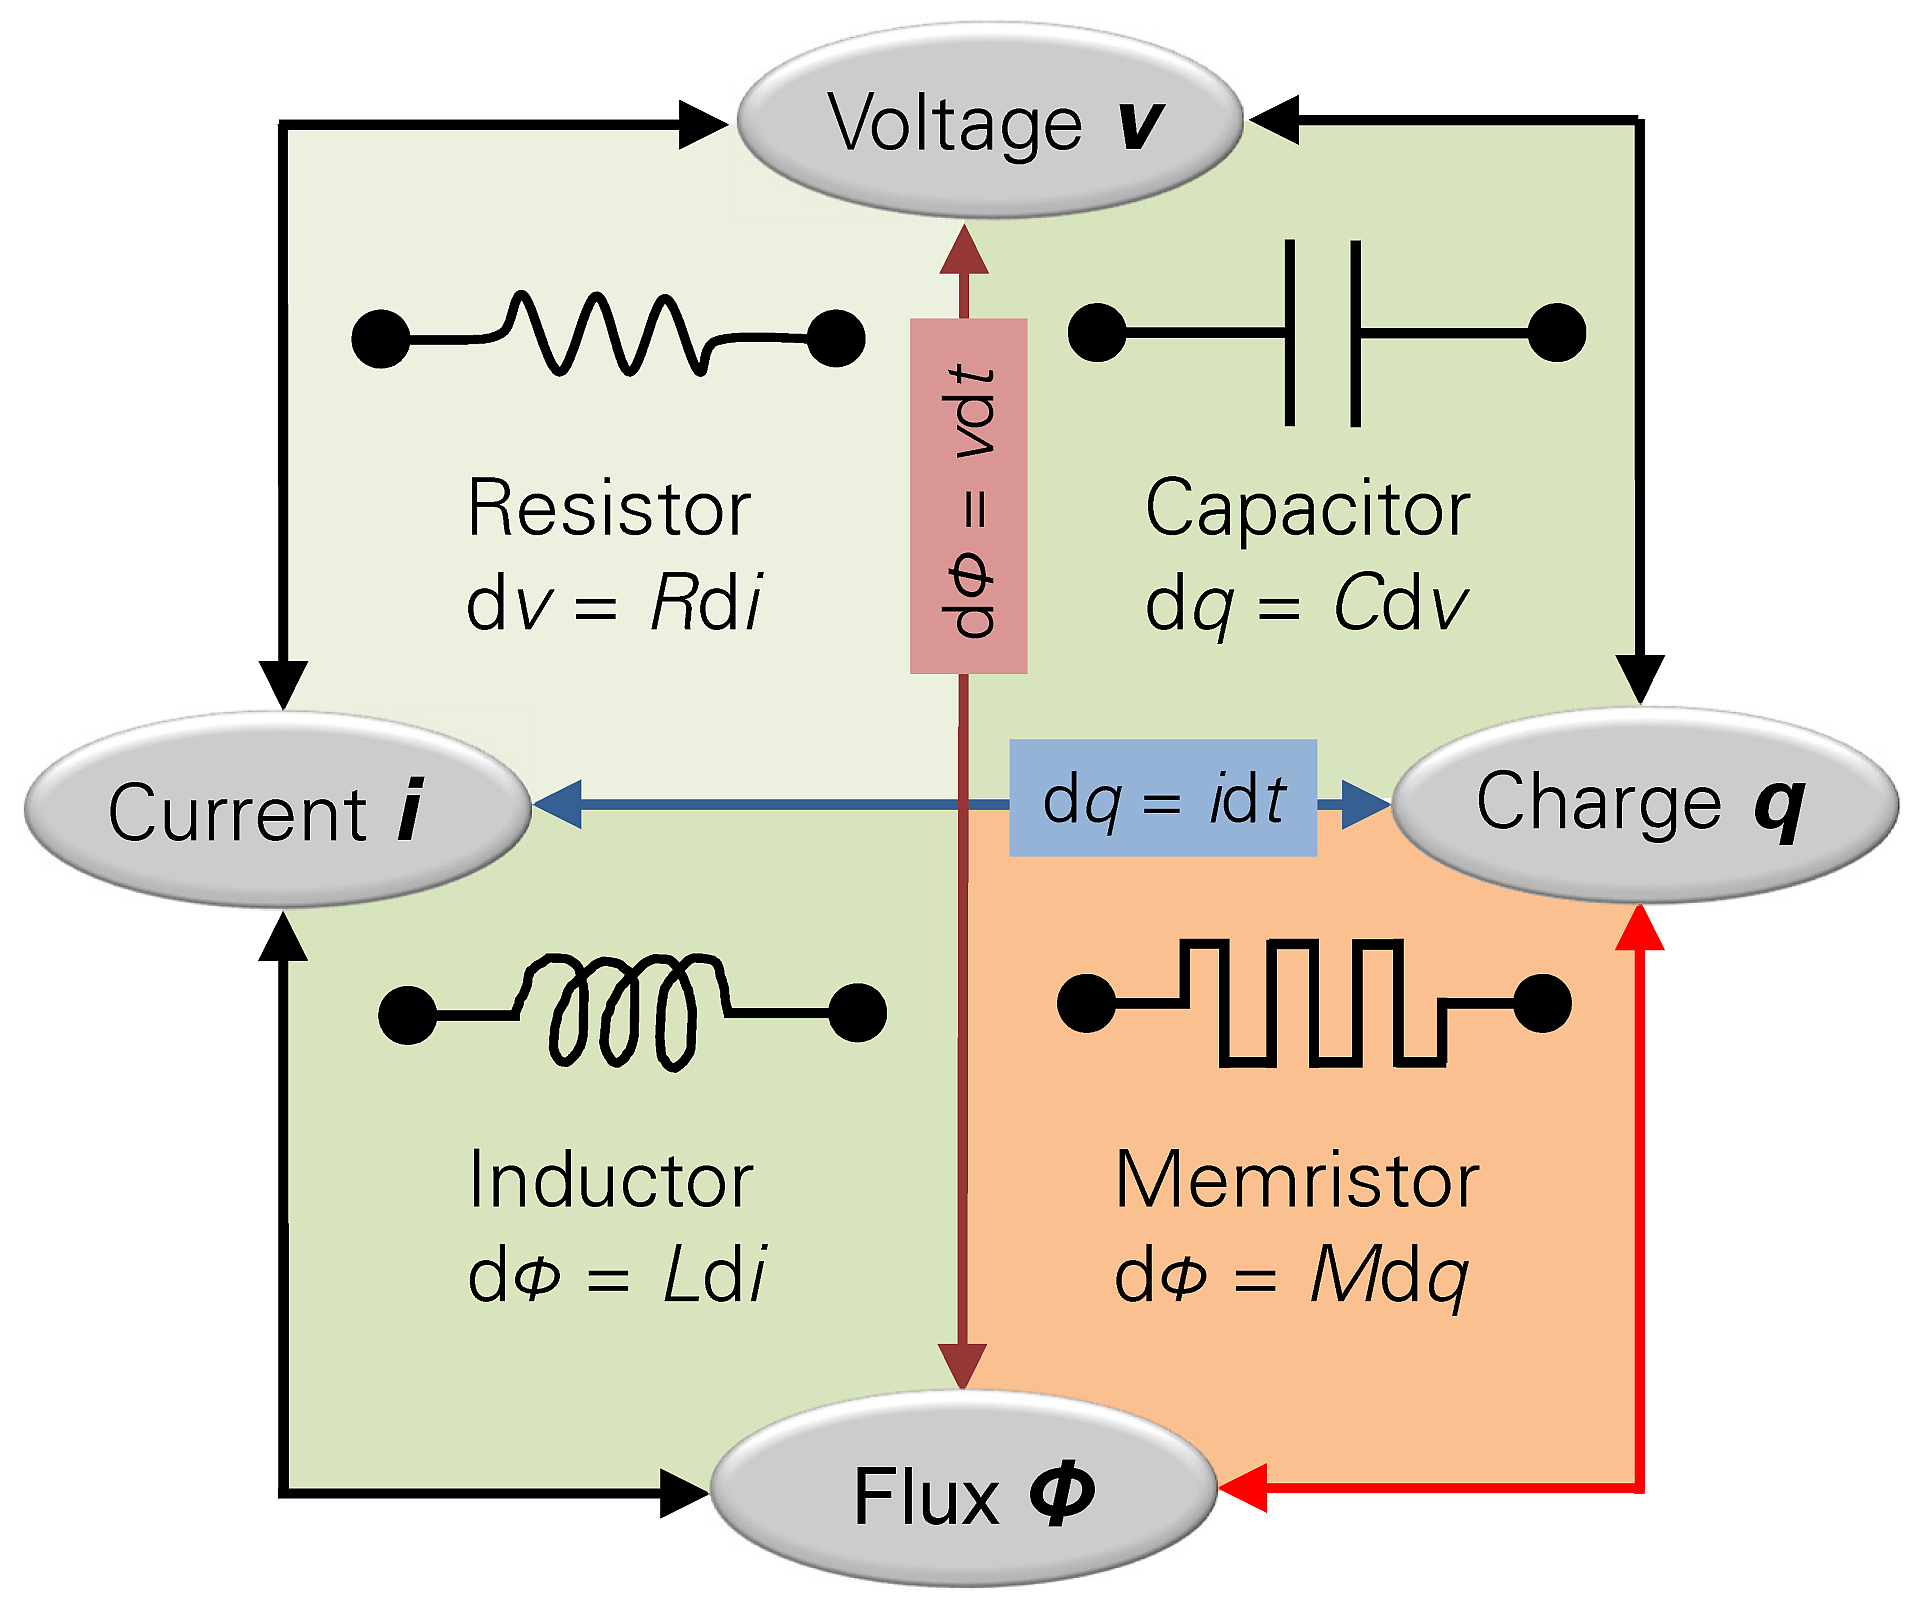
\includegraphics{Figures/Memristor.png}
  \caption{Fundamental passive components}
  \label{fig:fundComp}
\end{figure}

\subsubsection{Equations}
A memristor links the flux ($\phi$) and charge ($q$) and creates the memristance.
This memristance is defined with the following equation :
\begin{equation}
  M(q)=\frac{d\phi}{dq}
\end{equation}
It can be compared with the other fundamental components like resistor ($R(i)=\frac{dv}{di}$), capacitor ($\frac{1}{C(q)}=\frac{dv}{dq}$) and inductor ($L(i)=\frac{d\phi}{di}$).
We can then extract a more useful equation in an actual circuit :
\begin{equation}
  v(t)=M(q(t))\cdot i(t)
\end{equation}
Similarly, a memductance can be defined as such :
\begin{equation}
  W(\phi)=\frac{dq}{d\phi}
\end{equation}
A memristive device is slightly differently defined, it still uses a memristance, but here the memristance also depends on an internal state called $x$. This gives us this equation :
\begin{equation}
  v(t)=M(x,i)\cdot i(t)
\end{equation}
The internal state ($x$) is not linked to flux or charge in the case of a memristive device.\\
Once again, we can also define the memristive device using a memductance :
\begin{equation}
  i(t)=W(x,v)\cdot v(t)
\end{equation}
In all of the previous equations, $v$ is the voltage in Volt ($V$), $i$ is the current in Ampere ($A$), $\phi$ is the flux in Weber ($Wb$), $q$ is the charge in Coulomb ($C$), $M$ is the memristance in Ohm ($\Omega$) and $W$ is the memductance in Siesmens ($S$ or $\Omega^{-1}$).

\subsubsection{Behavior}
A memristor is defined as a non-linear two-terminal fundamental electrical component. It behaves as a resistance with memory (hence its name), meaning that it changes its resistance based on how much charge went through it. This enables us to manipulate the resistance of the component.
The huge benefit of memristors is the memory component, when you power it, it will have the resistance it had before.

Memristive devices have a similar behavior, the memristive device's resistance will change depending on the internal state ($x$). That internal state changes based on how much and how long voltage signals or currents are applied to the memristive device.

\subsubsection{Usage}
The main research for memristor usage is using them as ReRAM. The idea behind ReRAM is to use memristors as Non-Volatile memory. It uses two states of the device with known resistances ($R_{on}$ and $R_{off}$), giving it binary property. Reading the memory simply requires setting a voltage and reading the output current. It is better than current solutions (HDD, SSD) as it has a much lower latency. It is better than traditionnal DRAM because it keeps the information even when turned off. This makes ReRAM a good replacement for both RAM and HDDs/SSDs, thus eliminating Von Neumann bottleneck due to the Von Neumann architecture that is used in all modern computers.

They can also be used to set a resistance to be able to perform analog multiplication. Setting them in a crossbar array makes them a very strong candidate to be used in neuromorphic computing.

\subsection{Memristors Crossbar Array}\label{subsec:crossbar}

Setting memristors in a crossbar array to perform analog matrix multiplication typically called Multiply and Accumulate because of the nature of Matrix Multiplication. Figure \ref{fig:crossbar} shows what a typical crossbar array looks like.

\begin{figure}[H]
  \centering
  %\subfloat[Schematics]{\includesvg[width=.45\linewidth]{Figures/crossbar.svg}}\qquad
  \subfloat[Schematics]{
\includegraphics[width=.45\linewidth]{Figures/crossbar.eps}}%\qquad
  \hfill
  \subfloat[3 dimensional representation]{\includegraphics[width=.45\linewidth]{Figures/crossbar3D.jpg}}\\
  \caption{Memristor crossbar array}
  \label{fig:crossbar}
\end{figure}

It uses physical properties of electrical systems to perform analog computing. Lets use the circuit node in figure \ref{fig:crossNode} to explain the theory behind the memristor crossbar array.
\begin{figure}[H]
  \centering
  %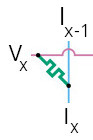
\includegraphics{Figures/crossbar-node.jpg}
  \includesvg[height=3.5cm]{Figures/crossbarNode.svg}
  \caption{Memristor crossbar node of the $i^{th}$ line and $j^{th}$ column}
  \label{fig:crossNode}
\end{figure}

First of all, a voltage is applied on the $i^{th}$ line, because every column is virtually grounded, the voltage applied to the memristor, of a set resistance of $R$, is $V_i$. As such and using Ohm's law, we know the the current flowing into the memristor is bound by the following equation :
\begin{equation}
  V_i = R\cdot I_{mem} \implies I_{mem} = V_i\cdot (\frac{1}{R})=I_{mem} = V_i\cdot G
\end{equation}
With $G$ being the conductance of memristor.
This line then joins the column where a current of $I_{i,j-1}$ is flowing, then according to kirchhoff's law the resulting current is :
\begin{equation}
  I_{j,i} = I_{j,i-1}+I_{mem} = I_{j,i-1} + V_i\cdot G
\end{equation}
By applying this process to the whole system we find that the current as the bottom of one column is :
\begin{equation}
  I_1=G_1\cdot V_1 + G_2\cdot V_2 + G_3\cdot V_3
\end{equation}
With $G_1$, $G_2$ and $G_3$ being the conductance of the 3 memristors in the first column.

This analog circuit removes the need to copy data from a main memory as the memristors themselves hold the value and the weights are then stored where the computation happens.

\subsection{memristor's model}
TODO
\subsection{LSTM}
\acp{LSTM} are a type of \ac{NN} used to analyze sequence of data. They are capable of predict data based of the previous results. \acp{LSTM} are part of \acp{RNN}. \acp{RNN} are different than feedfoward \acl{NN} because of their feedback connections. Meaning that the results from the last time step have an impact on the next time step.

\acp{LSTM} are able to forget information passed. This ability gave the uncommon name of \acl{LSTM} as it has both long and short term memory. This what gives \acp{LSTM} their use for sequence data. They can analyze the data and keep the information from the last time step to make a better decision afterwards. The most comprehensible example is considering a sentence. (TODO : find example)

An \ac{LSTM} is more complicated than just a simple feedforward \acl{NN}, they have several gates, which are all technically a \ac{NN} themselves. There is also a cell state which job is to hold a value for the next step.

\begin{figure}[H]
  \centering
  \includesvg[width=\textwidth]{Figures/lstmCellLatex.svg}
  \caption{LSTM Cell}
  \label{fig:lstmCell}
\end{figure}

Figure \ref{fig:lstmCell} shows the complexity of the \ac{LSTM} architecture. In an \ac{LSTM}, each gate is a different \ac{NN}.

An \ac{LSTM} works using different gates
\subsection{Dummy Subsection B}
\label{subsec:subsectionb}

State of Art Subsection B


\section{Main Contributions}
\label{sec:contributions}

In the thesis the following points will worked on in order to create, improve or clarify any of those topics :

\begin{itemize}
\item A script that can generate spice netlists for \acps{LSTM} or feed forward \aclp{NN} of any size and importing weights as resistance values from a specified file containing the architecture and the weights.
\item An \ac{LSTM} capable analog circuit.
\item Analog activation function circuit that supports \ac{tanh} and sigmoid ranges.
\item A \ac{VMM} capable analog circuit using a matrix of memristors.
\item Memory cells to store analog data for a short amount of time.
\item A python (tensorflow library) code to use piece wise functions, to reproduce in python the analog activation functions.
\item A way to run software simulation of different \acp{NN}.
\end{itemize}


\section{Thesis Outline}
\label{sec:int_outline}

Outline Section.

\cleardoublepage

% %%%%%%%%%%%%%%%%%%%%%%%%%%%%%%%%%%%%%%%%%%%%%%%%%%%%%%%%%%%%%%%%%%%%%%
% The State:
% %%%%%%%%%%%%%%%%%%%%%%%%%%%%%%%%%%%%%%%%%%%%%%%%%%%%%%%%%%%%%%%%%%%%%%
\fancychapter{State of the art}
\label{cap:state}

This chapter will go over the several subjects that need to be known in order to understand the thesis.

Math is the best way to universally describe all scientific models. For this reason, this chapter, and the thesis as whole, will contains equations.

It seems only logical to define all the tools that are going to be used in the thesis.

\begin{itemize}
  \item Vectors are displayed as $\overrightarrow{v}$ and are considered to be vertical matrixes, matrixes of size ($1\times n$) for vector of size $n$.
  \item $\overrightarrow{1}$ represent a vector that only contains ones of variable size.
  \item $\odot$ is used for the Hadamart product, that is the point wise multiplication of each element of the matrixes
  \item $\cdot$ is used in two cases :
    \begin{itemize}
      \item When used with scalars, it is the product of those scalars.
      \item When used with matrixes, it is the matrix product
    \end{itemize}
  \item $+$ is also used in two cases :
    \begin{itemize}
      \item When used with scalars, it is the sum of those scalars.
      \item When used with vectors (vertical matrixes), it is the point wise sum, basically adding each element to each other. The result is a vector of the same size.
    \end{itemize}
\end{itemize}


\section{\acl{AI}}\label{sec:ai}

\acf{AI} is very popular, and is getting more attention, being used as selling point by lots of services, the word is thrown around so much that it has lost its meaning. So let us see what are \acp{AI} exactly.

\ac{AI} is defined as theories and strategies used to simulate human intelligence, in other words, a computer or software that can take a decision by itself based on previously set rules. The definition is very wide and has lots of ways to be implemented.

The most promising type of \ac{AI} is machine learning, which in a broad sense means teaching the software to make decisions. It is defined as the use and development of computer systems that are able to learn and adapt without following explicit instructions, by using algorithms and statistical models to analyse and draw inferences from patterns in data.

\subsection{Machine learning}

In the last 10 years, the research concerning machine learning has considerably increased.

\begin{figure}[H]
  \centering
  \includesvg[width=\textwidth,pretex=\small]{ml.svg}
  \caption{Machine learning and its subsets}
  \label{fig:ml}
\end{figure}

\Cref{fig:ml} is a visual representation of machine learning and all the disciplines of machine learning. The thesis will focus, as the title implies, on the \aclp{RNN}.

\section{\aclp{NN}}\label{sec:nn}

\acfp{NN} are a set of units known as neurons. Those neurons are linked to each other with arcs known as synapses, thoses synapses each have a weight associated to them. The set of neurons interconnected with their synapses is what is called a \acl{NN}.
\Cref{fig:snn}, shows a simple representation of a \ac{NN}, the artificial neurons are the represented by the colored circles. On \cref{fig:snn} each arrow represent a synapse.

\begin{figure}[h!]
  \centering
  \includesvg[height=8cm]{NN_explained.svg}
  \caption{Simple \acl{NN}}
  \label{fig:snn}
\end{figure}

\acp{NN} contains several layers :

\begin{itemize}
  \item Input layer : This layer is simply the different inputs.
  \item Hidden layer : This layer can be (and usually is) wider than the one in figure \ref{fig:snn}. This is the layer that can be modified the most, by adding layers or increasing the amount of neurons in a layer.
  \item Output layer : This layer is where you can find the result from the \ac{NN}.
\end{itemize}

The weights of the synapses have to be multiplied with the previous neuron and then added to each other to produce the next stage. Using the names defined in figure \ref{fig:snn}, the output is linked to the input by \cref{eq:nnHid,eq:nnOut}. First, the hidden layers' neurons need to be computed (\cref{eq:nnHid}).

\begin{equation}\label{eq:nnHid}
  \begin{bmatrix}
    H_1\\ H_2\\ H_3\\ H_4\\
  \end{bmatrix}
  =
  \begin{bmatrix}
    w_h_{1,1} & w_h_{1,2} & w_h_{1,3}\\
    w_h_{2,1} & w_h_{2,2} & w_h_{2,3}\\
    w_h_{3,1} & w_h_{3,2} & w_h_{3,3}\\
    w_h_{4,1} & w_h_{4,2} & w_h_{4,3}\\
  \end{bmatrix}
  \cdot
  \begin{bmatrix}
    I_1\\ I_2\\ I_3\\
  \end{bmatrix}
\end{equation}

Similarly the output is computed like in \cref{eq:nnOut}

\begin{equation}\label{eq:nnOut}
  \begin{bmatrix}
    O_1\\ O_2
  \end{bmatrix}
  =
  \begin{bmatrix}
    w_o_{1,1} & w_o_{1,2} & w_o_{1,3} & w_o_{1,4}\\
    w_o_{2,1} & w_o_{2,2} & w_o_{2,3} & w_o_{2,4}\\
  \end{bmatrix}
  \cdot
  \begin{bmatrix}
    H_1\\ H_2\\ H_3\\ H_4\\
  \end{bmatrix}
\end{equation}

Those matrix multiplication are called \ac{VMM} because it is the result of the multiplication of a vector and a matrix, thus giving us another vector.

The model presented in \cref{fig:snn} is modular and can be scaled up as much as required. It is generally accepted that the more neurons a \ac{NN} has, the more complex the problems  it can solve can be.

\subsection{Training weights}

The weights values are obtained through training. In supervised learning, in order train the weights it is required to have a dataset of inputs/outputs values that are correct. The outputs are the target values, the values that the \ac{NN} needs to compute when being executed. The training starts once the weights have been initialized (usually randomly picked values). The training is an iteravtive process, each iteration being called an epoch. Each of those epoch usally consists of the following steps :

\begin{enumerate}
  \item Run the \ac{NN} to get an output vector.\label{step:restart}
  \item Measure the error (known as loss) by comparing the current prediction with the targeted output using the chosen error algorithm (\ac{RMSE}, \ac{MSE}, etc).
  \item Run the backpropagation algorithm to change each individual weight.
\end{enumerate}

The number of epochs required depends on the complexity of the problem the \ac{NN} is solving.

Once trained, the \ac{NN} can be tested by feeding the \ac{NN} input data it hasn't seen before.

\section{\acl{RNN}}\label{sec:rnn}

\acp{RNN} are, as the name suggests, a type of \ac{NN} using recurrent connections. They are a \ac{NN} with at least one cycle within the structure, outputs of previous time step are used as input for the next time step, these outputs are generally known are hidden states. Those feedback connections are the main difference from feedforward \ac{NN}.

This type of \ac{NN} is used when dealing with an unknown amount of inputs. Especially useful when treating time series \cite{rnn}. Example of \acp{RNN} uses are speech recognition, automatic language translation \cite{gru} and shape recognition, especially for handwriting recognition.

Traditionnal \acp{RNN} have the ability to model sequential events by propagating through time, for example forward and backward propagation. This is achieved by connecting these sequential events with the hidden state like in \cref{eq:rnn}.

\begin{equation}\label{eq:rnn}
  \overrightarrow{h_t}=f(\overrightarrow{x_t},\overrightarrow{h_{t-1}})
\end{equation}

The hidden state ($\overrightarrow{h_t}$) carries all the past informations for the next time step. It also serves as the output of the \ac{RNN}.

They are trained the same way \ac{NN} are, measuring the error, backpropagating and adjusting the weights accordingly.

\subsection{Simple \acl{RNN}}

The simple \ac{RNN} works just like a \ac{tanh} activated feedforward \ac{NN} with a feedback connection.

\begin{figure}[H]
  \centering
  \begin{minipage}{\columnwidth}
    \subfloat[\acs{RNN} cell\label{fig:rnnCell}]{\includesvg[width=\textwidth,pretex=\large]{rnn/rnnCell.svg}}
  \end{minipage}
  \begin{minipage}{\columnwidth}
    \subfloat[Legend\label{leg:cells}]{\includesvg[width=\textwidth,pretex=\large]{cellsLegend.svg}}
  \end{minipage}
  \caption{}
\end{figure}

\Cref{eq:srnn} shows the equation that the simple \ac{RNN} runs at every time step.

\begin{equation}\label{eq:srnn}
  \overrightarrow{h_t}=tanh([\overrightarrow{x_t},\overrightarrow{h_{t-1}}]\cdot w + \overrightarrow{b})
\end{equation}

Where $t\in\mathbb{N}^*$ is the time index, $w$ the weight matrix, $\overrightarrow{b}$ the bias vector, $\overrightarrow{x_t}$ the input vector and $\overrightarrow{h_{t}}$ the hidden state of the \ac{RNN}.

\subsection{Vanishing gradient problem}

The Vanishing gradient problem is a problem that comes when dealing with time dependent data \cite{vanishGrad}. When a big amount of time dependent data is fed to the \ac{RNN}, the weights cannot be updated properly. The older the data, the lower it will impact how much the weight must change. Rendering the old input data almost useless. That is the reasom why, simple \acp{RNN} must be used with relatively short time series.

Some \acp{RNN} were designed to tackle this issue. This is the case of the \ac{LSTM} and \ac{GRU} which were created with internal mechanisms to regulate the flow of information and gradients.

\section{\acs{LSTM}}\label{sec:lstm}
\acfp{LSTM} are a type of \ac{RNN} used to analyze sequences of data. They are capable of predicting data based on previous data points.

The first \ac{LSTM} was invented in 1997 by Hochreiter and Schmidhuber \cite{firstLSTM}. \acp{LSTM} changed a lot through the years to become what they are now.

\acp{LSTM} was created to fix the vanishing gradient problem. \acp{LSTM} alleviate this issue by adding a cell state, this state gives it the ability to choose what input is important and which one is not, thus giving it a long term memory. This ability gave the uncommon name of \acl{LSTM} as it has both long and short term memory. This is what makes \acp{LSTM} adequate for sequence data. They can analyze the data and keep the information from the last time step to make a better decision afterwards. The most comprehensible example is considering a sentence. %TODO : find example)

An \ac{LSTM} is more complicated than just a simple feedforward \acl{NN}, it has several gates, which all compute a \ac{VMM}. There is also a cell state whose job is to hold a value for the next step.

\begin{figure}[H]
  \centering
  \includesvg[width=\textwidth,pretex=\large]{lstm/lstmCell.svg}
  \label{fig:lstmCell}
  \caption{\acs{LSTM} cell, adapted from \cite{wikiLSTM}}
\end{figure}

\Cref{fig:lstmCell} shows the complexity of the \ac{LSTM} architecture. In an \ac{LSTM}, each gate is a different \ac{NN} and then activated with either a \ac{tanh} or a sigmoid activation function. Each input to the cell is a vector.
Those vectors are of varying sizes depending on several factors. For example, both $h_t$ and $c_t$ are of the same size as the number of hidden states (sometimes referred to as cell state) for any $t\geq 0$.
The input vector ($x_t$) is of size of the sample we want to feed for each time step.

\subsection{Equations}

The equations of an LSTM are quite unusual.
Let's start with the more classic gate equations. They are the ones that behave like the more classic \ac{NN}.
The input (\cref{eq:inputG}), forget (\cref{eq:forgetG}) and output (\cref{eq:outputG}) gates are described below.


\begin{equation}\label{eq:inputG}
  \overrightarrow{i_t}=\sigma ([\overrightarrow{x_{t_1}},\overrightarrow{h_{t-1}}]\cdot w_i + \overrightarrow{b_i})
\end{equation}
\begin{equation}\label{eq:forgetG}
  \overrightarrow{f_t}=\sigma ([\overrightarrow{x_{t_1}},\overrightarrow{h_{t-1}}]\cdot w_f + \overrightarrow{b_f})
\end{equation}
\begin{equation}\label{eq:outputG}
  \overrightarrow{o_t}=\sigma ([\overrightarrow{x_{t_1}},\overrightarrow{h_{t-1}}]\cdot w_o + \overrightarrow{b_o})
\end{equation}

Where ($w_i$,$\overrightarrow{b_i}$), ($w_f$,$\overrightarrow{b_f}$) and ($w_o$,$\overrightarrow{b_o}$) are the pair of weights matrixes and bias vectors for the input, forget and output gates respectively. $\overrightarrow{x_t}$ is the input vector and $\overrightarrow{h_t}$ is the hidden state vector.

The next equation describes the candidate cell state (\cref{eq:candCell}), that will next be used to compute the cell state (\cref{eq:cellS}).

\begin{equation}\label{eq:candCell}
  \overrightarrow{\tilde{c}_t}=tanh([\overrightarrow{x_{t_1}},\overrightarrow{h_{t-1}}]\cdot w_c+ \overrightarrow{b_c})
\end{equation}
\begin{equation}\label{eq:cellS}
  \overrightarrow{c_t}=\overrightarrow{f_t}\odot \overrightarrow{c_{t-1}} + \overrightarrow{i_t} \odot \overrightarrow{\tilde{c}_t}
\end{equation}

Where $w_c$ and $\overrightarrow{b_c}$ are the weights matrix and bias vector for the candidate cell state.

The final step of the \ac{LSTM} is to compute the hidden state (\cref{eq:hiddenS}).
\begin{equation}\label{eq:hiddenS}
  \overrightarrow{h_t}=\overrightarrow{o_t}\odot tanh(\overrightarrow{c_t})
\end{equation}

We set $x_1$ as the first input and define $\overrightarrow{h_0}$ as a zero only vector.

\subsection{Usage}

Using \ac{LSTM} can be a bit tricky. Due to its sequential nature, it takes several time steps. Every hidden state ($h_t$) is passed to the next time step as an input. This hidden state can be used to compute an output at any time step $t$. \Cref{fig:lstmUse} shows a visual representation of an \ac{LSTM} going from the current time step to the following time step.

\begin{figure}[H]
  \centering
  \includesvg[width=\textwidth]{lstm/lstmUse}
  \caption{Unfolded \acs{LSTM}, legend in \cref{leg:cells}}
  \label{fig:lstmUse}
\end{figure}

\subsection{Variants}

\acp{LSTM} come in a few different flavors of implementations. Usually, when \acp{LSTM} are mentionned, the version used is the \ac{NP} version. This is the most common version as those are the equations described on the wikipedia page \cite{wikiLSTM} and used in libraries like Keras \cite{Keras} or PyTorch \cite{PyTorch}. In fact, there are at least 8 other variations of \acp{LSTM} \cite{nbLSTM}.
The difference between them varies from one to the other, some of them are detailled next.

\subsubsection{Vanilla \ac{LSTM}}
This variant of the \ac{LSTM} was originally the only \ac{LSTM} network, hence its name. It differs from the classic \ac{LSTM} with its use of peephole weights, hence the name of the classic \ac{LSTM} being \acl{NP}. The Vanilla \ac{LSTM} is thus defined by the following equations \cite{vanillaLSTM, nbLSTM} :

\begin{equation}\label{eq:inputGVanilla}
  \overrightarrow{i_t}=\sigma ([\overrightarrow{x_{t_1}},\overrightarrow{h_{t-1}}]\cdot w_i + \overrightarrow{b_i} +\overrightarrow{c_{t-1}}\odot \overrightarrow{p_f})
\end{equation}
\begin{equation}\label{eq:forgetGVanilla}
  \overrightarrow{f_t}=\sigma ([\overrightarrow{x_{t_1}},\overrightarrow{h_{t-1}}]\cdot w_f + \overrightarrow{b_f}+\overrightarrow{c_{t-1}}\odot \overrightarrow{p_i})
\end{equation}
\begin{equation}\label{eq:ouputGVanilla}
  \overrightarrow{o_t}=\sigma ([\overrightarrow{x_{t_1}},\overrightarrow{h_{t-1}}]\cdot w_o + \overrightarrow{b_o}+\overrightarrow{c_{t}}\odot \overrightarrow{p_o})
\end{equation}

With $\overrightarrow{p_f}$, $\overrightarrow{p_i}$ and $\overrightarrow{p_o}$ being the peephole weights vectors. Their size is the same as the size of the hidden state vector ($\overrightarrow{h_t}$). $\odot$ is the pointwise multiplication operator.

The equations that have not been rewritten simply stay the same.

\subsubsection{\acf{FGR} \ac{LSTM}}
This variant of the \ac{LSTM} is the most complex of all. This is due to the amount of feedback connections. This is basically a more complex version of the Vanilla \ac{LSTM}. The modified equations are :

\begin{equation}\label{eq:inputGFGR}
  \overrightarrow{i_t}=\sigma ([\overrightarrow{x_{t_1}},\overrightarrow{h_{t-1}}]\cdot w_i  + \overrightarrow{i_{t-1}}\cdot R_{ii} + \overrightarrow{f_{t-1}}\cdot R_{if} + \overrightarrow{o_{t-1}}\cdot R_{io} + \overrightarrow{b_i} +\overrightarrow{c_{t-1}}\odot \overrightarrow{p_i})
\end{equation}
\begin{equation}\label{eq:forgetGFGR}
  \overrightarrow{f_t}=\sigma ([\overrightarrow{x_{t_1}},\overrightarrow{h_{t-1}}]\cdot w_f  + \overrightarrow{i_{t-1}}\cdot R_{fi} + \overrightarrow{f_{t-1}}\cdot R_{ff} + \overrightarrow{o_{t-1}}\cdot R_{fo} + \overrightarrow{b_f} +\overrightarrow{c_{t-1}}\odot \overrightarrow{p_f})
\end{equation}
\begin{equation}\label{eq:ouputGFGR}
  \overrightarrow{o_t}=\sigma ([\overrightarrow{x_{t_1}},\overrightarrow{h_{t-1}}]\cdot w_o + \overrightarrow{i_{t-1}}\cdot R_{oi} + \overrightarrow{f_{t-1}}\cdot R_{of} + \overrightarrow{o_{t-1}}\cdot R_{oo} + \overrightarrow{b_o} +\overrightarrow{c_{t-1}}\odot \overrightarrow{p_o})
\end{equation}

With $R_{fi}$ being the weight matrix of the input feedback connection to compute the forget gate, and the same goes for the other weight matrixes.

Once again, the equations that have not been rewritten are unchanged.

\subsubsection{Other small variants}

\begin{itemize}
  \item Removing the activation function from the Vanilla \ac{LSTM} for :
    \begin{itemize}
      \item the candidate cell and thus becomes $ \overrightarrow{\tilde{c}_t}=(w_c\cdot[\overrightarrow{x_{t-1}},\overrightarrow{h_{t-1}}] + \overrightarrow{b_c}) $, this is called the \ac{NIAF}
      \item the output of the previous cell state and thus becomes $ \overrightarrow{h_t}=\overrightarrow{o_t}\odot \overrightarrow{c_t} $, and is called \ac{NOAF}
    \end{itemize}
  \item Using units instead of the respective gates :
    \begin{itemize}
      \item \ac{NIG} : $\overrightarrow{i_t}=1$
      \item \ac{NOG} : $\overrightarrow{o_t}=1$
      \item \ac{NFG} : $\overrightarrow{f_t}=1$
    \end{itemize}
\end{itemize}

\section{\acs{GRU}}\label{sec:gru}
The \acf{GRU} is another type of \ac{RNN}. It is also known to reduce the effect of the vanishing gradient problem. It was first introduced to improve translation techniques \cite{gru}.

The \ac{GRU} is very often compared to the \ac{LSTM}, being sometimes assimilated as a type of \ac{LSTM} \cite{nbLSTM}. Their performance was found to be very similar in most situations \cite{gruVSlstm}, making those two types of \acp{RNN} coexistant in the modern machine learning world.

There are two versions of the \ac{GRU}, both are found on the internet, they are known as the encoder and decoder version \cite{gru}. They were originally designed to encode the message to translate and then decode in the translation. PyTorch only supports the decoder version \cite{gruPyTorch}, while the Keras library supports both \cite{gruKeras} chosen by changing an argument.

\subsection{Encoder \ac{GRU}}

The encoder \ac{GRU} is the version of the \ac{GRU} most widely described on the internet. It contains an update gate (\cref{eq:updateG}), a reset gate (\cref{eq:resetG}), a candidate activation gate (\cref{eq:candActivG}). The hidden state is then computed (\cref{eq:gruHidG}) using the previous results.

\begin{equation}\label{eq:updateG}
  \overrightarrow{z_t}=\sigma ([\overrightarrow{x_t},\overrightarrow{h_{t-1}}] \cdot w_z + \overrightarrow{b_z})
\end{equation}
\begin{equation}\label{eq:resetG}
  \overrightarrow{r_t}=\sigma ([\overrightarrow{x_t},\overrightarrow{h_{t-1}}] \cdot w_r + \overrightarrow{b_r})
\end{equation}
\begin{equation}\label{eq:candActivG}
  \overrightarrow{\hat{h_t}}=tanh(\overrightarrow{x_t}\cdot w_{hx}+(\overrightarrow{r_t}\odot\overrightarrow{h_{t-1}}) \cdot w_{hh} + \overrightarrow{b_h})
\end{equation}
\begin{equation}\label{eq:gruHidG}
  \overrightarrow{h_t}=(\overrightarrow{1}-\overrightarrow{z_t})\odot \overrightarrow{h_{t-1}} + \overrightarrow{z_t}\odot \overrightarrow{\hat{h_t}}
\end{equation}

Where ($w_z$,$\overrightarrow{b_z}$), ($w_r$,$\overrightarrow{b_r}$),($w_{hx}$,$w_{hh}$,$\overrightarrow{b_h}$) are the weights matrixes and bias vectors for the update, reset and candidate activation gates respectively.

A visual representation of the encoder \ac{GRU} cell is available in \cref{fig:encoderGruCell}.

\begin{figure}[H]
  \centering
  \includesvg[width=\textwidth,pretex=\large]{gru/encoderCell.svg}
  \label{fig:encoderGruCell}
  \caption{Encoder \acs{GRU} cell, legend in \cref{leg:cells}}
\end{figure}

Sometimes the \cref{eq:gruHidG} can be found in another form (\cref{eq:gruHidG1})\cite{gruPyTorch}. This, however, has no impact on the final results, it means the weights are going to be trained differently for the update gate.

\begin{equation}\label{eq:gruHidG1}
  \overrightarrow{h_t}=\overrightarrow{z_t}\odot \overrightarrow{h_{t-1}} + (\overrightarrow{1}-\overrightarrow{z_t})\odot \overrightarrow{\hat{h_t}}
\end{equation}

\subsection{Decoder \ac{GRU}}

The decoder \ac{GRU}, while being less described, is the version used in pyTorch, which is getting very popular.

The candidate activation gate (\cref{eq:candActivG1}) is the only difference from the encoder \ac{GRU}.

\begin{equation}\label{eq:candActivG1}
  \overrightarrow{\hat{h_t}}=tanh(\overrightarrow{x_t}\cdot w_{hx}+ \overrightarrow{b_{hx}}+\overrightarrow{r_t}\odot[\overrightarrow{h_{t-1}} \cdot w_{hh} + \overrightarrow{b_{hh}}])
\end{equation}

A visual representation of the decoder \ac{GRU} cell can be found in \cref{fig:decoderGruCell}.

\begin{figure}[H]
  \centering
  \includesvg[width=\textwidth,pretex=\large]{gru/decoderCell.svg}
  \label{fig:decoderGruCell}
  \caption{Decoder \acs{GRU} cell, legend in \cref{leg:cells}}
\end{figure}

\subsection{Similarities with \ac{LSTM}}

While the \ac{GRU} is its own type of \ac{RNN}, it has been compared and assimilated to an \ac{LSTM} \cite{nbLSTM}. Indeed, the subtype of \ac{LSTM} it has been associated with is called the \ac{CIFG} \ac{LSTM}. If the input and forget gates are combined into one ($\overrightarrow{f_t}=\overrightarrow{1}-\overrightarrow{i_t}$), they can be assimilated as the update gate of the \ac{GRU}. The reset gate would then be the \ac{LSTM}'s output gate.

\Cref{eq:lstmGru0,eq:lstmGru1,eq:lstmGru2,eq:lstmGru3,eq:lstmGru4} are the \ac{GRU}'s equations with the \ac{LSTM}'s names.

\begin{equation}\label{eq:lstmGru0}
  \overrightarrow{f_t}=\sigma ([\overrightarrow{x_t},\overrightarrow{h_{t-1}}] \cdot w_f + \overrightarrow{b_f})
\end{equation}
\begin{equation}\label{eq:lstmGru1}
  \overrightarrow{o_t}=\sigma ([\overrightarrow{x_t},\overrightarrow{h_{t-1}}] \cdot w_o + \overrightarrow{b_o})
\end{equation}
\begin{equation}\label{eq:lstmGru2}
  \overrightarrow{i_t}=\overrightarrow{1}-\overrightarrow{f_t}
\end{equation}
\begin{equation}\label{eq:lstmGru3}
  \overrightarrow{\tilde{c_t}}=tanh(\overrightarrow{x_t}\cdot w_{cx}+(\overrightarrow{o_t}\odot\overrightarrow{h_{t-1}}) \cdot w_{ch} + \overrightarrow{b_c})
\end{equation}
\begin{equation}\label{eq:lstmGru4}
  \overrightarrow{h_t}=(\overrightarrow{i_t})\odot \overrightarrow{h_{t-1}} + \overrightarrow{f_t}\odot \overrightarrow{\tilde{h_t}}
\end{equation}

Differences between the two \acp{RNN} are :
\begin{itemize}
  \item The \ac{GRU} has no output activation function.
  \item The \ac{GRU} has combined hidden state and cell state.
  \item The \ac{GRU}'s candidate hidden state is point wise multiplied with the reset gate before passing into the dense layer.
\end{itemize}

\section{Memristors}
\label{sec:memristors}

Memristors are the lesser known fourth fundamental passive component of electronics, among resistors, capacitors and inductor.
It was first theorized in 1971 by L. Chua from UC Berkeley, in \cite{TheoMemristor}. The name comes from the blend of \textit{memory} and \textit{resistance}.
The theory behind this component was extracted from a missing component to link the four fundamental circuit variables, voltage ($v$), charge ($q$), current ($i$) and flux ($\phi$). \Cref{fig:fundComp} shows the four fundamental variables are on each side of the square, with the ones on opposite sides being linked by the following equations :
\begin{equation}
  d\phi = v\cdot dt
\end{equation}

\begin{equation}
  dq = i\cdot dt
\end{equation}

Resistors, capacitors and inductors were already very established and well known component, so it was theorized that a fourth device should then exists to physically link flux ($\phi$) and charge ($q$).  The flux in this case is not a magnetic flux and is defined as such : $ d\phi=v\cdot dt \Rightarrow \phi =  \int v \,dt  $.\\
The component stayed theoretical until 2008 when it's been implemented in a physical device for the first time \cite{memristorFab}. It took 37 years to have an actual working device.\\
There is then an extention of this theoretical device to another, the memristive device. It was theorized in 1976 by L. Chua and S. M. Kang \cite{memrestiveDev}. The difference between the memristor and the memristive device is its internal behavior. Memristive device are commonly referred to as memristor as well.

\begin{figure}[H]
  \centering
  \includesvg[width=0.55\textwidth]{memristor/memristor}
  \caption{Fundamental passive components}
  \label{fig:fundComp}
\end{figure}

\subsection{Equations}
A memristor links the flux ($\phi$) and charge ($q$) and creates the memristance.
This memristance is defined with the following equation :
\begin{equation}
  M(q)=\frac{d\phi}{dq}
\end{equation}
It can be compared with the other fundamental components like resistor ($R(i)=\frac{dv}{di}$), capacitor ($\frac{1}{C(q)}=\frac{dv}{dq}$) and inductor ($L(i)=\frac{d\phi}{di}$).
We can then extract a more useful equation in an actual circuit :
\begin{equation}
  v(t)=M(q(t))\cdot i(t)
\end{equation}
Similarly, a memductance can be defined as such :
\begin{equation}
  W(\phi)=\frac{dq}{d\phi}
\end{equation}
A memristive device is slightly differently defined, it still uses a memristance, but here the memristance also depends on an internal state called $x$. This gives us this equation :
\begin{equation}\label{eq:memristiveDev}
  v(t)=M(x,i)\cdot i(t)
\end{equation}
The internal state ($x$) is not linked to flux or charge in the case of a memristive device.\\
Once again, we can also define the memristive device using a memductance :
\begin{equation}
  i(t)=W(x,v)\cdot v(t)
\end{equation}
In all of the previous equations, $v$ is the voltage in Volt ($V$), $i$ is the current in Ampere ($A$), $\phi$ is the flux in Weber ($Wb$), $q$ is the charge in Coulomb ($C$), $M$ is the memristance in Ohm ($\Omega$) and $W$ is the memductance in Siesmens ($S$ or $\Omega^{-1}$).

\subsection{Behavior}

A memristor is defined as a non-linear two-terminal fundamental electrical component. It behaves as a resistance with memory (hence its name), meaning that it changes its resistance based on how much charge went through it. This enables us to manipulate the resistance of the component.
The huge benefit of memristors its ability to retain its internal resistance, the device can left without power for a long period of time (retention time of minimum 10 years according to \cite{memRetention}). When the device is powered backup, it will have the same resistance it had before.

Memristive devices have a similar behavior, the memristive device's resistance will change depending on the internal state ($x$). That internal state changes based on how much and how long voltage signals or currents are applied to the memristive device.

\subsection{Usage}
The main research for memristor usage is using them as ReRAM. The idea behind ReRAM is to use memristors as Non-Volatile memory. It uses two states of the device with known resistances ($R_{on}$ and $R_{off}$), giving it binary property. Reading the memory simply requires setting a voltage and reading the output current. It is better than current solutions (HDD, SSD) as it has a much lower latency. It is better than traditionnal DRAM because it keeps the information even when turned off. This makes ReRAM a good replacement for both RAM and HDDs/SSDs, thus eliminating Von Neumann bottleneck due to the Von Neumann architecture that is used in all modern computers.

They can also be used to set a resistance to be able to perform analog multiplication. Setting them in a crossbar array makes them a very strong candidate to be used in neuromorphic computing.

\section{Memristors Crossbar Array}\label{sec:crossbar}

Setting memristors in a crossbar array allows to perform analog \ac{VMM}, also called Multiply and Accumulate. This circuit works great for this use as all the computation is done almost instantly and using physics laws. \Cref{fig:crossbar} shows what a typical crossbar array looks like.

\begin{figure}[H]
  \centering
  \subfloat[Schematics, inspired from \cite{xbarFigures}]{\includesvg[width=.45\linewidth]{crossbar/crossbar}}%\qquad
  \hfill
  \subfloat[3 dimensional representation, from \cite{xbarFigures}]{\includegraphics[width=.45\linewidth]{crossbar/crossbar3D.jpg}}\\
  \caption{Memristor crossbar array}
  \label{fig:crossbar}
\end{figure}

It uses physical properties of electrical systems to perform analog computing. In what follows I will use the circuit node in \cref{fig:crossNode} to explain the theory behind the memristor crossbar array.
\begin{figure}[H]
  \centering
  \includesvg[height=3.5cm]{crossbar/node}
  %\def\svgheigth{3.5cm}
  %\input{crossbar/node.pdf_tex}
  \caption{Memristor crossbar node of the $k^{th}$ line and $j^{th}$ column}
  \label{fig:crossNode}
\end{figure}

First of all, a voltage is applied on the $k^{th}$ line, because every column is virtually grounded, the voltage applied to the memristor, of a set resistance $\symR_k$, is $\symv_k$. As such and using Ohm's law, we know that the current flowing into the memristor ($\symi_{k}$) is bound by the following equation :

\begin{equation}
  \symv_k = \symR_k\cdot \symi_{k} \Rightarrow \symi_{k} = \symv_k\cdot (\frac{1}{\symR_k})= \symv_k\cdot \symG_k
\end{equation}
With $\symG_k$ being the conductance of memristor, defined as $\symG_k=\frac{1}{\symR_k}$.

This line then joins the column where a current of $\symi_{j,k-1}$ is flowing, then according to Kirchhoff's current law the resulting current is :
\begin{equation}
  \symi_{j,k} = \symi_{j,k-1}+\symi_{k} = \symi_{j,k-1} + \symv_k\cdot \symG_k
\end{equation}
By applying this process to the whole system we find that the current at the bottom of one column is :
\begin{equation}
  \symi_1= \symG_1\cdot \symv_1 +  \symG_2\cdot \symv_2 +  \symG_3\cdot \symv_3
\end{equation}
With $\symG_1$, $\symG_2$ and $\symG_3$ being the conductance of the 3 memristors in the first column.

Using such an analog circuit is a huge gain in time, for two main reasons :

\begin{itemize}
  \item By being analog, this circuit allows for analog computations which are much faster than their digital counterparts. As explained in this section, the circuit only uses physical properties of the different components and can compute large \acp{VMM} in a very short amount of time.
  \item The other advantage of such a system is the use of the memristors, that make the need to copy data from another memory useless as the memristors have a long term memory themselves. This is one of the ways to break down the Von Neumann bottleneck.
\end{itemize}

\section{Memristor's model}\label{sec:model}

They are several ways to model a memristor \cite{memristorFab,memTEAMmodel, memVTEAMmodel, memristorSpiceModels}. The way the memristor works depends on the materials used to fabricate the memristor. Each type of memristor has slightly different behavior. Models were thus created to simulate, as accurately as possible, the memristor in electrical circuit simulation software such as \textbf{Cadence}'s \textit{virtuoso} or SPICE.

Some examples of memristor's model are :

\begin{itemize}
  \item \acf{LIDM}, the model of the first memristor \cite{memristorFab}.
  \item \acf{STBM}, is another model of the $TiO_x$ memristor created in 2008 by \textbf{HP} \cite{memristorFab, memristorSpiceModels}.
  \item \acf{TEAM}, is a model that can easily adapt to several types of memristive devices while focusing on fast computation \cite{memTEAMmodel}.
  \item \acf{VTEAM}, is a later improvement of the \ac{TEAM}. The internal resistance depends on voltage, unlike \ac{TEAM} which depends on current \cite{memVTEAMmodel}.
\end{itemize}

The \ac{VTEAM} being the most versatile model, its implementation would fit most memristor types.

\subsection{Equations}

It's been established that the internal resistance also depends on an internal state $x$ (\cref{eq:memristiveDev}).

\begin{equation}
  \frac{dx}{dt}=f(x,v)
\end{equation}

Where $v$ is the voltage, $t$ is time and $f$ is a function.

The function $f$ is described in its simplest form as in \cref{eq:funcDesc}.

\begin{equation}\label{eq:funcDesc}
  f(x,v)=g(x)\cdot s(v)
\end{equation}

Where $g$ is the window function and $s$ the sensitivity function.

\begin{itemize}
  \item The window function delimits the operational boundaries of the memristor.
  \item The sensitivity function, also known as voltage sensitivity describes the effect of voltage on the internal state's variations.
\end{itemize}

The model is based on previous work \cite{memCadenceModel} that aims to reproduce as many memristive device types. They have chosen to use the resistive state ($R$) as the internal state \cite{memModelOrigin}. Based on this assumption the \cref{eq:memModel0,eq:memModel1} are extracted from the memristive device. This model is of course very basic and ignores some physical dependencies such as temperature.

\begin{equation}\label{eq:memModel0}
  i(R,v)=
  \begin{cases}
    \frac{a_p}{R}\cdot sinh(b_p\cdot v) & v\ge 0\\
    \frac{a_n}{R}\cdot sinh(b_n\cdot v) & v<0\\
  \end{cases}
\end{equation}

\begin{equation}\label{eq:memModel1}
  \frac{dR}{dt}=f(R,v)=s(v)\cdot g(R,v)
\end{equation}

The sensitivity function was chosen to be a voltage-dependent exponential function, like described in \cref{eq:memModel2}.

\begin{equation}\label{eq:memModel2}
  s(v)=
  \begin{cases}
    A_p\cdot (e^{t_p\cdot |v|}-1)& v>0\\
    A_n\cdot (e^{t_n\cdot |v|}-1)& v<0\\
    0 &  v=0\\
  \end{cases}
\end{equation}

The window function used is a state-dependent quadratic function as shown in \cref{eq:memModel3}.

\begin{equation}\label{eq:memModel3}
  g(R,v)=
  \begin{cases}
    (R-r_p(v))^2& v>0\\
    (R-r_n(v))^2& v<0\\
    0 &  v=0\\
  \end{cases}
\end{equation}

Where $r_p$ and $r_n$ are voltage dependent in a polynomial manner. They represent the boundaries of the state variable. All the other parameters in \cref{eq:memModel0,eq:memModel1,eq:memModel2,eq:memModel3} that haven't been declared are free fitting variables. They have to be set depending on the type of memristor used.

\subsection{Verilog-A integration}

The model now needs to be adapted to work as Verilog-A code.
Verilog-A is a hardware desciption language, very popular in the industry for its simplicity and flexibility when using it with circuit simulator such as \textbf{Cadence}'s \textit{virtuoso}.

The focus of this specific implementation will be the resistance range $[20k\Omega, 120k\Omega]$. The boundaries functions are found in \cref{eq:memModel4}.

\begin{equation}\label{eq:memModel4}
  \begin{cases}
    r_p(v)= r_{p,0} + r_{p,1}\cdot v& v>0\\
    r_n(v)= r_{r,0} + r_{n,1}\cdot v& v\le 0\\
  \end{cases}
\end{equation}

Where $r_{p,0}$, $r_{p,1}$, $r_{n,0}$ and $r_{n,1}$ are free fitting variables that need to be extracted from the physical device.

The changes of resistive states from the initial resistance ($R_0$) are computed by \cref{eq:memModel5} extracted from \cite{memCadenceModel}. It uses the bias voltage ($V_b$) of the pulse applied to the memristor. The pulse has a duration of $t$.

\begin{equation}\label{eq:memModel5}
  R(t)_{|V_b} =
  \begin{cases}
    \frac{R_0+s(V_b)\cdot r_p(V_b)\cdot(r_p(V_b)-R_0)\cdot t}{1+s(V_b)\cdot (r_p(V_b)-R_0)\cdot t} & V_b>0, R<r_p(V_b)\\
    \frac{R_0+s(V_b)\cdot r_n(V_b)\cdot(r_n(V_b)-R_0)\cdot t}{1+s(V_b)\cdot (r_n(V_b)-R_0)\cdot t} & V_b\le 0, R>r_n(V_b)\\
    R_0 & else\\
  \end{cases}
\end{equation}

The final Verilog-A code is available at \cref{apsec:memModel}.

\subsection{Behavior}

The model was tested then tested. As with physical memristors, it has a threshold voltage value from which its resistive states starts changing. This threshold value is $V_{read}$. For this specific model the threshold voltage is set to $V_{read}=500mV$.

Every pulse is composed of 2 parts and last for a total of $1 ms$ :
\begin{itemize}
  \item The reading of the resistive state, by applying a triangular wave that in bound by the threshold value $V_{read}$.
  \item The writing to the memristor. During this part the resistive state will change. This is done by apply a square wave of variable width ($t_{\Delta}$) with a set bias voltage ($V_{bias}$).
\end{itemize}

\begin{figure}[H]
  \centering
  \includesvg[width=\textwidth]{memristor/input.svg}
  \label{graph:memInput}
  \caption{Pulse shape graph}
\end{figure}

The \cref{graph:memInput} is the visual representation of what each pulse, the value is read during the first half of the pulse.

The resistive state of the memristor changes depending on the pulse width ($t_{\Delta}$) and the bias voltage ($V_{bias}$) used for each pulse.

\begin{figure}[H]
  \centering
  \includesvg[width=\textwidth]{memristor/memPulseChange.svg}
  \label{graph:pulseChange}
  \caption{Memristor's resistive state under different pulses width (Fixed bias voltage $V_{bias}=1.8V$)}
\end{figure}

The effect of the pulse width variation is shown in \cref{graph:pulseChange}. Indeed, the larger the pulse widths, the faster the internal resistance reaches the bounding resistance (\cref{eq:memModel4}). The bounding resistance being the same as all curve use the same bias voltage ($V_{bias}=1.8V$), the curves will all eventually reach the max resistance.

\begin{figure}[H]
  \centering
  \includesvg[width=\textwidth]{memristor/memVoltChange.svg}
  \label{graph:voltChange}
  \caption{Memristor's resistive state under different voltages (Fixed pulse width $t_{\Delta}=100\mu s$)}
\end{figure}

The voltage dependence of the memristor's model is described in \cref{graph:voltChange}. The influence of the bias voltage is, as \cref{eq:memModel3,eq:memModel4} show, the way to change the resistance range of the memristor, until the physical limit is reached of course. Applying higher voltage also allows to reach a set resistance faster as the slopes are bigger the higher the bias voltage gets.

The resistive state can also be lowered by applying negative voltages.TODO

%\subsection{\acf{LIDM}}

%The \ac{LIDM} is the model of the first memristor eveer created, it was created to fit the behavior of the $TiO_x$ memristor they had just fabricated \cite{memristorFab}. The device, of width $D$, has two parts. The doped part and the undoped


\cleardoublepage

% %%%%%%%%%%%%%%%%%%%%%%%%%%%%%%%%%%%%%%%%%%%%%%%%%%%%%%%%%%%%%%%%%%%%%%
% Dummy Chapter:
% %%%%%%%%%%%%%%%%%%%%%%%%%%%%%%%%%%%%%%%%%%%%%%%%%%%%%%%%%%%%%%%%%%%%%%

% %%%%%%%%%%%%%%%%%%%%%%%%%%%%%%%%%%%%%%%%%%%%%%%%%%%%%%%%%%%%%%%%%%%%%%
% The Introduction:
% %%%%%%%%%%%%%%%%%%%%%%%%%%%%%%%%%%%%%%%%%%%%%%%%%%%%%%%%%%%%%%%%%%%%%%
\fancychapter{The design}
\label{cap:design}

In this chapter, I'm going to describe the different design decisions taken during the study of the thesis.

The system will be working with a $V_{dd}$ of $1.8V$. Such a value was chosen because this is a low power system.

The way values are encoded in the analog system will be descibed here as it serves for the entire thesis.
In order for the system to support negative numbers we're going to use a $V_{cm}$ set to $\frac{V_{dd}}{2}$. That means that $V_{cm}=\frac{V_{dd}}{2}=0.9V$. This $V_{cm}$ will then describe a zero. A step of one was chosen to be $0.1V$ in the analog circuit.
\Cref{tab:valConv} shows the conversions from a real number to it's voltage equivalent.

\begin{table}[H]
  \centering
  \begin{tabular}{|c|c|}
    \hline
    \rowcolor{gray}
    Real value & Voltage \\
    \hline
    $0$ & $0.9V$ \\
    \hline
    $1$ & $1.0V$ \\
    \hline
    $x$ & $V(x)=\frac{x}{10}+V_{cm}$\\
    \hline
    $real(v)=(v-0.9)\cdot 10$ & $v$\\
    \hline
  \end{tabular}
  \caption{Real/Voltage Conversion Table.}
  \label{tab:valConv}
\end{table}

Since the system cannot reach voltage outside of the operating range with the intended behavior, the voltage is then restricted to $V\in [0,1.8]$. This means that the range of real value that the systems can handle is $x\in [-9,9]$.

Any data inputed in the analog system should have been previously checked to make sure it stays in the range of accepted values.

In order to create a fully functional \ac{LSTM} or \ac{GRU} circuit, there are a few components that are required.

An analog activation function circuit to have an analog equivalent to the activation function necessary to the good behavior of \acp{LSTM} and \acp{GRU}.

A memory cell to allow to store the analog value from one time step to the next.

A circuit for the crossbar array, to have a more general circuit that can easily be adapted.

Other, less significant, components required for the circuits to work.

\section{The activation functions}
\label{sec:af}

Activation functions play a great role in the results obtained \cite{af}. It is the reason why making good Activation function circuits is fundamental. Of course the easy way would be to simply design a hard sigmoid (\cref{apsec:hardFunc}), the issue being that the hard sigmoid is much worse than the regular sigmoid, especially for regression problems \cite{hardSigm}. The same goes for the \ac{tanh} and hard \ac{tanh} functions.

Designing an analog activation function as close to the original is very important for the final result's quality.

\begin{table}[H]
  \centering
  \begin{tabular}{|c|c|c|}
    \hline
    \rowcolor{gray}
    Parameter & Sigmoid & \ac{tanh} \\
    \hline
    $V_1$ & \multicolumn{2}{c|}{$1.1V$}\\
    \hline
    $V_2$ & \multicolumn{2}{c|}{$635mV$}\\
    \hline
    $V_3$ & $0.8V$ & $550mV$\\
    \hline
    $i_{dc}$ & \multicolumn{2}{c|}{$150uA$}\\
    \hline
    $w$ & \multicolumn{2}{c|}{$900nm$}\\
    \hline
    $l$ & \multicolumn{2}{c|}{$60nm$}\\
    \hline
    $R_1$ & \multicolumn{2}{c|}{$5k\Omega$}\\
    \hline
    $R_2$ & \multicolumn{2}{c|}{$10k\Omega$}\\
    \hline
    $R_3$ & $2k\Omega$ & $4k\Omega$\\
    \hline
  \end{tabular}
  \caption{Circuits parameters}
  \label{tab:afPar}
\end{table}

Here, $w$ and $l$ are, respectively, the width and length of the two NMOS of the circuit.

\subsection{Circuit}

The circuit used is the same as the one in \cite{thesisRef}, the circuit is the one shown in \cref{circt:af}. The technology used being different, all the parameters had to be determined empirically to best fit a sigmoid shape. The parameters can be found in \cref{tab:afPar}.

Due to the nature of the functions we want to generate, we will use the same circuit for both a sigmoid and a \ac{tanh} like functions. The two different functions are generated by changing two parameters.

The functions generated are the same shape and only differ by their output range.

\begin{figure}[H]
  \centering
  \includesvg[width=\textwidth]{activation/afCircuit}
  \caption{Activation functions circuit}
  \label{circt:af}
\end{figure}

\subsection{Symbols}
The symbols for the sigmoid and the \ac{tanh} are separated for better understanding.

\begin{figure}[H]
  \centering
  \hspace*{0.8cm}
  \subfloat[Sigmoid symbol]{\includesvg[height=2.5cm]{activation/sigmoidSymbol}}%
  \hfill
  \subfloat[\ac{tanh} symbol]{\includesvg[height=2.5cm]{activation/tanhSymbol}}%
  \hspace*{0.8cm}
  \caption{Activation functions symbols with the input and output pins on either side depending on the flow of the current for better readability}
  \label{fig:afSymbol}
\end{figure}

The approximate onChip area of this circuit is :

\begin{equation}
  A_{af}=2\cdot A_{R_1} + 2\cdot A_{CMOS} + 5\cdot A_{R_2} + A_{R_3} +2\cdot A_{opAmp}
\end{equation}
With $A_{CMOS} = w\cdot l = 9\cdot 10^{-7} \cdot 6 \cdot 10^{-8} = 5.4 \cdot 10^{-14} m^2$
TODO : Finish calc

In order to combine the the onChip area of both the sigmoid and \ac{tanh} activation functions, it is assumed that the variation of area taken by the resistor ($R_3$) is negligible compared to th overall area.

\subsection{Usage}

This circuit outputs a voltage that depends on the input voltage passed on. The relation between the two is shown in \cref{fig:afGraph}. The graph also shows the \ac{RMSE} of each graph compared to the ideal result.

Note that the actual output of the circuit in \cref{circt:af} is inverted arround $V_{cm}$ a simple circuit such as the one shown in  (TODO show circuit in annex) does inverts the

\begin{figure}[H]
  \centering
  \includesvg[width=\textwidth]{activation/afGraph}
  \caption{Input/Output graph of the activation function circuit for both sigmoid and \acs{tanh} functions}
  \label{fig:afGraph}
\end{figure}

These functions are still a bit different from the original functions (especially for the \ac{tanh}). However that doesn't matter too much as the trainning will be happening within the final circuit, all weights will be set in the circuit. This is the reason why such a difference doesn't matter. As long as the curves have the similar shape, the result won't be drastically affected.

\section{Memory cells}
\label{sec:memcell}

The memory cell is a circuit that is able to store an analog value for a limited time. It works using capacitors that have the ability to store a voltage for a short period of time.

\subsection{Circuit}

The circuit is shown in \cref{circt:memcell}. The value/voltage is trapped in the capacitor using \ac{CMOS} switches.

\begin{figure}[H]
  \centering
  \includesvg[width=\textwidth]{memcell/memCircuit}
  \caption{Memory cell circuit}
  \label{circt:memcell}
\end{figure}

The cirucit has a two \ac{CMOS} switches design to avoid voltage leakage through the swicthes. The system has voltage leakage when only one \ac{CMOS} swicth, and thus leads to a large memory leak. This is due to the high voltage difference between the two sides of the \ac{CMOS} swicth. Using two \ac{CMOS} switches allows for this difference to be mitigated (\cref{fig:memcellLoss}).

\begin{figure}[H]
  \centering
  \includesvg[width=\textwidth]{memcell/data-loss}
  \caption{Memory conservation in a memory cell with 1 \ac{CMOS} switch vs 2 \ac{CMOS} swicthes}
  \label{fig:memcellLoss}
\end{figure}

\subsection{Symbol}

The symbol for this circuit is designed to show a capacitor because it is its memory mechanism.

\begin{figure}[H]
  \centering
  \includesvg[height=2.5cm]{memcell/memcellSymbol}
  \caption{Memory cell symbol with the input enable pin (top) and the output enable pin (bottom). The left and right pins are interchangebly the input and ouput for the sake of readability}
  \label{circt:memcell}
\end{figure}

For this circuit the approximate onChip area is :

\begin{equation}
  A_{memcell}=8\cdot A_{CMOS}+2\cdot A_{inv}+A_{opAmp}+A_{cap}
\end{equation}

With $A_{CMOS} = w\cdot l = 2\cdot 10^{-7} \cdot 6 \cdot 10^{-8} = 1.2 \cdot 10^{-14} m^2$

\subsection{Usage}

This circuit is pretty straight forward, when the input enable pin is high (up to $V_{dd}$), then the first switch is open and the capacitor is being charged, if it is low, then the switch is closed and the capacitor keeps the voltage and thus the analog data. When the output enable is high, the buffer (\cref{apsec:buffer}) forwards the voltage stored in the capactor to the output pin without emptying the capacitor.

\begin{figure}[H]
  \centering
  \begin{tikztimingtable}
    Input data & x6D{$x_1$}6D{$x_2$}6D{$x_3$}x \\
    Input enable & xL2H2L3H7L2HLx\\
    Output enable & x3L2H4L5H1L3Hx\\
    Memory & xU4D{$x_1$}10D{$x_2$}3D{$x_3$}x \\
    Output data & x3U2D{$x_1$}4U5D{$x_2$}U3D{$x_3$}x \\
    \extracode
    \tablerules
    %\draw (0,0) circle (2pt); % Origin
    \begin{pgfonlayer}{background}
      \vertlines[help lines]{0.6,18.6}
      %\vertlines[red]{1.6,5.6,15.6}
      %\vertlines[blue]{3.6,9.6,15.6}
    \end{pgfonlayer}
  \end{tikztimingtable}
  \caption{Time diagram that shows the logic of the memory cell}
  \label{tim:memcell}
\end{figure}

\section{Voltage-driven crossbar circuit}
\label{sec:xbarCircuit}

The crossbar circuit theory has already been explained in the \cref{sec:crossbar}. This section describes how the crossbar circuit is actually implemented. The final circuit is the one in \cref{circt:xbar}. The circuit depends on three parameters :

\begin{itemize}
  \item $n_i$ : The number of input for our crossbar array (not including bias for a more general circuit).
  \item $n_o$ : The number of parallel output for our crossbar array.
  \item $n_s$ : The serial size of our crossbar system.
\end{itemize}

\begin{figure}[H]
  \centering
  \includesvg[width=\textwidth]{crossbar/crossbarUse}
  \caption{Circuit of the crossbar array used in the final system ($n_i$, $n_o$, $n_s$)}
  \label{circt:xbar}
\end{figure}

The parallel and serial are explained later (\cref{subsec:serpar}).

The enable flags ($e_j,\forall j\in[\![ 0,n_s]\!]$ and similarly $\overline{e_j}$) are there to show when the \ac{CMOS} switches are open, the states of those flags is shown in \cref{tim:serpar}.

\subsection{Two memristors per synapse}
\label{subsec:doubleMem}

We could choose between one or two memristor per synapse. Using two memristor per synapse doubles the area but doubles the weight range (\cref{tab:synapses}) and allows to easily use negavite weights. The output voltage will be centered around $V_{cm}$ and be compliant with the standard set in \cref{tab:valConv}.

This design is the one that is used in \cite{doubleMem}. Let's assume that a given memristor has a resistance range of $R\in[R_{min},R_{max}]$, that means its conductance range is $ G \in [ G_{min}, G_{max}]$ (with $ G_{min}= \frac{1}{R_{max}}$ and $ G_{max}= \frac{1}{R_{min}}$). This design works using two \ac{opAmp} connected to $V_{cm}$ with the positive pin and the negative pin to the output of the crossbar array. \Cref{eq:doubleMem0,eq:doubleMem1,eq:doubleMem2} are describing how this architecture works. A simplified version of the double memristors per synapse circuit is also available in \cref{circt:doubleMem}.

\begin{figure}[H]
  \centering
  \includesvg[width=\textwidth,pretex=\scriptsize]{crossbar/doubleMem}
  \caption{Simplified circuit of a double memristor per synapse architecture}
  \label{circt:doubleMem}
\end{figure}

Using $x_k$ as the voltage for the input line $k$. The highest \ac{opAmp} is identified as $opAmp_0$ and the lowest $opAmp_1$.

For the sake of simplicity, the following equations considers the ground to be $V_{cm}$.

\begin{equation}
  \label{eq:doubleMem0}
  V_{opAmp_0}=-R_r\cdot i_+
\end{equation}
\begin{equation}
  \label{eq:doubleMem1}
  i_{R_f}=i_-+\frac{V_{opAmp_0}}{R_r}=i_--i_+
\end{equation}
\begin{equation}
  \label{eq:doubleMem2}
  V_{opAmp_1}=y_0=-R_f\cdot(i_--i_+)=R_f\cdot(i_+-i_-)=R_f\cdot\sum_{k=0}^n( G_{k+}- G_{k-})\cdot x_k
\end{equation}
With $i_+=\sum_{k=0}^n G_{k+}\cdot x_k$ and $i_-=\sum_{k=0}^n G_{k-}\cdot x_k$.


\begin{table}[H]
  \centering
  \begin{tabular}{|c|c|c|}
    \cline{2-3}
    \rowcolor{gray}
    \multicolumn{1}{c|}{\cellcolor[HTML]{FFFFFF}} & Two memristors per synapse & One memristor per synapse \\
    \hline
    Maximum weight & $ G_{max}- G_{min}$ & $ G_{max} -\overline{ G}$\\
    \hline
    Minimum weight & $ G_{min}- G_{max}$ & $ G_{min} -\overline{ G}$\\
    \hline
    Range & $2\cdot( G_{max}- G_{min})$&$ G_{max}- G_{min}$\\
    \hline
  \end{tabular}
  \caption{Synaptic weights precision (extracted from \cite{doubleMem})}
  \label{tab:synapses}
\end{table}

\subsection{Serialization}
\label{subsec:serpar}

This circuit has the option to be serialized with varying degrees. The idea of serializing the circuit came from \cite{thesisRef}. Serializing the circuit reduces the number of components required and thus reduces the final onChip area. Serializing the system increases the time it takes to compute the output.

Serializing the system means not computing all values of the output vector at the same time, but instead computing group by group, the groups' size are $n_o$. The first output group is computed during $e_0$ and the $i^{th}$ group is computed during $e_i$. The timing of when the outputs are available is found in \cref{tim:serpar}. Those flag control the \ac{CMOS} swicthes present in \cref{circt:xbar}, the switches control which output group is outputed.

The \ac{CMOS} switches are here to open the necessary input gates when the output is required, the \ac{CMOS} switches are controlled as in \cref{tim:serpar}.

\begin{figure}[H]
  \centering
  \begin{tikztimingtable}
    $e_0$ & x2H2L N(A1) L N(A2) 2L N(A3) L N(A4) 2Lx\\
    $e_1$ & x2L2H N(B1) L N(B2) 2L N(B3) L N(B4) 2Lx\\
    $e_i$ & x4L N(C1) L N(C2) 2H N(C3) L N(C4) 2Lx\\
    $e_{n_s-1}$ & x4L N(D1) L N(D2) 2L N(D3) L N(D4) 2Hx\\
    %foo & 2L N(A1)  4H N(A2) L\\
    \extracode
    \node[gap, at={($(A1|-A2)!0.5!(A2)$)}];
    \node[gap, at={($(A3|-A4)!0.5!(A4)$)}];
    \node[gap, at={($(B1|-B2)!0.5!(B2)$)}];
    \node[gap, at={($(B3|-B4)!0.5!(B4)$)}];
    \node[gap, at={($(C1|-C2)!0.5!(C2)$)}];
    \node[gap, at={($(C3|-C4)!0.5!(C4)$)}];
    \node[gap, at={($(D1|-D2)!0.5!(D2)$)}];
    \node[gap, at={($(D3|-D4)!0.5!(D4)$)}];
    \tablerules
    %\draw (0,0) circle (2pt); % Origin
    \begin{pgfonlayer}{background}
      \vertlines[help lines]{0.55,10.55}
      %\vertlines[red]{1.6,5.6,15.6}
      %\vertlines[blue]{3.6,9.6,15.6}
    \end{pgfonlayer}
  \end{tikztimingtable}
  \caption{Enable flags timing for any value of $n_s$ in a single time step}
  \label{tim:serpar}
\end{figure}

When the system is used fully in parallel, the \ac{CMOS} switches are not required can then be removed to lower the final onChip area.

%TODO understand better \subsection{Sneak path problem}
\subsection{Symbol}
The symbol (\cref{sym:xbar}) defined for the voltage based memristor crossbar array used in this thesis is more compact and helps the readability of the circuits that require a crossbar array. It depends on several parameters, the number of inputs ($n_i$), the number of outputs ($n_o$) and the serial size ($n_s$).

\begin{figure}[H]
  \centering
  \includesvg[height=2.5cm]{crossbar/xbarSymbol}
  \caption{Symbol used for the crossbar array, the input pin is a bus of size $n_i$ and the output pin is a bus of size $n_o$}
  \label{sym:xbar}
\end{figure}

The approximate onChip area for the crossbar circuit depends on the previously defined parameters.

\begin{equation}
  A_{xbar}(n_i,n_o,n_s)=
  \begin{cases}
    2\cdot n_i\cdot n_o \cdot A_{memristor}+n_o\cdot(2\cdot[A_{opAmp}+A_{R_r}]+A_{R_f})& n_s=1\\
    \begin{array}{2}
      2\cdot n_i\cdot n_o \cdot n_s\cdot A_{memristor}+2\cdot A_{CMOS}\cdot n_o\cdot n_s\\
      +n_o\cdot(2\cdot[A_{opAmp}+A_{R_r}]+A_{R_f})
    \end{array}
    & \forall n_s>1\\
  \end{cases}
\end{equation}

With $A_{CMOS}=w\cdot l$.

\subsection{Usage}

\subsubsection{Input voltages}

The input voltages must be monitored very carefuly in order not to accidentally change a memristor's internal resistance. Indeed, memristors have a voltage threshold ($V_{read}$) above which the internal resistance changes \cite{memristorSpiceModels,memCadenceModel,memTEAMmodel,memVTEAMmodel}. This means that the input voltages must follow the inequality in \cref{eq:memThres}.

\begin{equation}\label{eq:memThres}
  |V_{mem}|= |x_i-V_{cm}|\le V_{read}
\end{equation}

Where $V_{mem}$ is the terminal voltage of a memristor.

\subsubsection{Dense layer}

A dense layer is simply a \ac{VMM}. This means that a dense layer in a \ac{NN} can be assimilated with a crossbar array. Dense layers are mostly used as by fully parallel voltage-driven crossbar array in this thesis to keep the timing simple, otherwise the timing of the enable flags, and later on the \ac{LSTM}'s memory cells (\cref{sec:lstm}), would get too complicated.

\subsubsection{Resistors vs Memristors}

In this work, the analog system will be simulated for the inference of the \ac{NN}, thus the weights will not have to change during the simulation. Because the weights are represented in the analog circuit by the internal resistances of the memristors, the memristors can be replaced by resistors with a set resistance for the simulation.

\section{Inverter}
\label{sec:inv}

This section simply describes a very well know electrical component, the inverter. When it a voltage of $V_{dd}$ is applied to the input, the output is grounded and the same goes for the other way around.

\begin{figure}[H]
  \centering
  \hspace*{2.5cm}
  \subfloat[Inverter's circuit]{\label{circt:inv}\includesvg[height=3cm]{inverter/invCircuit}}%
  \hfill
  \subfloat[Inverter's symbol]{\label{sym:inv}\includesvg[height=2.5cm]{inverter/invSymbol}}%
  \hspace*{1.5cm}
  \caption{}
  \label{fig:inv}
\end{figure}

Like mentionned, the circuit for the inverter is very straight forward (\cref{circt:inv}). The symbol is nothing fancy as well as it is the classic symbol (\cref{sym:inv}) for such a circuit.

The approximate onChip area for the inverter is :
\begin{equation}
  \symA_{inv}=2\cdot \symA_{CMOS}
\end{equation}

With $\symA_{CMOS}= w\cdot l=2\cdot 10^{-7}\cdot6\cdot10^{-8} =1.2\cdot10^{-14}m^2$.

The onChip area of the inverter is then $\symA_{inv}=2.4\cdot10^{-14}m^2$.

\section{Verilog models}
\label{sec:models}

Due to a lack of time, some of the more common component were not designed by me but instead were simulated using a Verilog model. Verilog is a hardware description laguage very popular in the industry. The only components that use a verilog model are the voltage multiplier and the \ac{opAmp}.

\subsection{Operational amplifier}\label{subsec:opamp}

This component is the very famous \ac{opAmp}. This specific component wasn't designed for the thesis, it required a current range that didn't allow to use ones already made by members of the research group. The choice was then to use a verilog-A model, and then design one if time allows it.

\begin{equation}
  \label{eq:opAmp}
  V_{out}=\mu \cdot (V_+-V_-)
\end{equation}

\Cref{eq:opAmp} is the equation used in the verilog-A model. It makes it so it behaves like an ideal \ac{opAmp}. For this thesis $\mu$ has been set to $\mu=10^5$.

\subsection{Voltage multiplier}\label{subsec:voltmult}

This component while far less popular than the latter, is just as useful for our specific use. It allows us to multiply, as its name implies, two voltages. It is used to compute the pointwise multiplications of the \ac{LSTM} (\cref{fig:lstmCell}).

However this part is tricky. Indeed, because of the voltage conversion (\cref{tab:valConv}), the equation needs to take that into consideration. The final equation needs to be \cref{eq:finalVoltMult} in order to have $1\cdot 1=1$ ($V_{in_1}\cdot V_{in_2}=1V$, with $V_{in_1}=V_{in_2}=1V$)

\begin{equation}\label{eq:finalVoltMult}
  V_{out}=10\cdot(V_{in_1}-V_{cm})\cdot (V_{in_2}-V_{cm}) + V_{cm}
\end{equation}

This is taken care of using in reality two parts, the actual voltage multiplier (\cref{eq:voltMult}) and a non inverting amplifier (\cref{eq:invAmp}), the circuit of which is available in \cref{apsec:invAmp}.

\begin{equation}\label{eq:voltMult}
  V_{voltMult}=-(V_{in_1}-V_{cm})\cdot (V_{in_2}-V_{cm}) + V_{cm}
\end{equation}
\begin{equation}\label{eq:invAmp}
  V_{out}=-(V_{voltMult}-V_{cm})\cdot10+V_{cm}
\end{equation}

Where $V_{out}$ is the output voltage the inverting amplifier (\cref{apsec:invAmp}), $V_{voltMult}$ is the out voltage of the voltage multiplier itself and $V_{in_1}$ and $V_{in_2}$ are the input voltages.

The \cref{eq:voltMult} is assumed possible because of the actual voltage multiplier's datasheet available at \cite{actualVoltMult}.

\subsection{Symbols}

The symbols for those two components are the ones in \cref{sym:models}.

\begin{figure}[H]
  \centering
  \hspace*{2cm}
  \subfloat[\ac{opAmp}'s symbol\label{sym:opAmp}]{\includesvg[height=2.5cm]{models/opAmpSymbol}}%
  \hfill
  \subfloat[Voltage multiplier's symbol\label{sym:voltMult}]{\includesvg[height=2.5cm]{models/voltMultSymbol}}%
  \hspace*{2cm}
  \caption{Symbols used for the verilog-A components}
  \label{sym:models}
\end{figure}

The \ac{opAmp} uses its classic symbol (\cref{sym:opAmp}) while the voltage multiplier uses a custom symbol (\cref{sym:voltMult}).

\section{\ac{LSTM} analog implementation}\label{sec:lstmCircuit}

\subsection{Circuit}

This section describes the circuit of an \ac{LSTM} with an input vector of size $n_i$, a $n_h$ hidden states, a serial size of $n_s$ and $n_{ts}$ time steps. $n_o=n_h/n_s$ is going to be used for future references in this section. In order for the crossbar array to be used $n_o$ must be an integer, in other words, $n_s$ must divide $n_h$. The circuit (shown in \cref{circt:lstm}) is pretty complex and contains numerous parts that require explaination.

\begin{figure}[H]
  \centering
  \includesvg[width=\textwidth,pretex=\tiny]{lstm/lstmCircuit}
  \caption{\ac{LSTM} circuit}
  \label{circt:lstm}
\end{figure}

The system is built using crossbar array (\cref{sec:xbarCircuit}) with ($n_i+n_h+1$,$n_o$, $n_s$) as parameters.

First of all, the different vectors and variables present in the schematic have to be described :

\begin{itemize}
  \item $\overrightarrow{x_t}$ : This is the input vector for the \ac{LSTM} circuit at time $t$. It has a size of $n_i$.
  \item $\overrightarrow{h_t}$ : This is the hidden layer vector for the feedback connections, it is defined as $\overrightarrow{h_t}=(\overrightarrow{h_{t,i}}) \forall i\in [\![0,n_o-1]\!]$, with $\overrightarrow{h_{t,i}}=(h_{t,i,j}) \forall j\in [\![0,n_s-1]\!]$.
  \item $\overrightarrow{z_t}$ is the input of the crossbar but not the input of the \ac{LSTM}. This vector is there to lighten the informations on the schematic (\cref{circt:lstm}). $\overrightarrow{z_t}$ is defined by $\overrightarrow{z_t}=(\overrightarrow{x_t},\overrightarrow{h_{t-1}},b)$.
  \item $e_{j,0}$ and $e_{j,1}$ are two enable flags that respectively represent the first and second half of $e_j$.
  \item $e_{in}$ and $e_{out}$ are the flags used to enable the hidden state values to go to the input (feedback connection) or to the output of the circuit.
  \item $e_{next}$ is the enable flag on in between two time steps.
  \item $R_{amp0}$ and $R_{amp1}$ are the two resistances used to amplify the output voltage of the voltage multipliers. The ratio of the resistances value must of $\frac{R_{amp1}}{R_{amp0}}=10$. The resistances must stay arround the values of the resistances used around the circuit, especially those of the memristors.
\end{itemize}

The wires coming into the crossbar are a bus of size $n_i+n_h+1$ and the output of the crossbar is a bus of size $n_o$ (\cref{sym:xbar}). This is why everything in the system apart from the crossbar arrays is only shown once in \cref{circt:lstm} but in reality those components are present $n_o$ times. Those extra components are needed in order for the parallel channels to work.

\subsection{Doubling memory cells}

\subsubsection{Feedback hidden states}

In order for the system to work in serial mode, the memory cells of the output need to be doubled. This is done in \cref{circt:lstm}, and allows for the hidden states to be saved for the next stage. Indeed, if using the system in serial mode with only one line of memory cells, the old hidden state ($\overrightarrow{h_{t-1}}$) is slowly overwritten by the current hidden state ($\overrightarrow{h_t}$). As soon as the first $n_o$ serial values are computed, they are going to override the old ones, still required for the following serial values. \Cref{tim:lstmMemcell} shows that the value in the memory cell changes too early in the cycle and gives a bad input for the next serial values. The value given to the input of the \ac{LSTM} should always be the old hidden state ($\overrightarrow{h_{t-1}}$).

\begin{figure}[H]
  \centering
  \begin{tikztimingtable}
    $e_{n_s-1}$ & 3H8Lx \\
    $e_0$ & 3L4H4Lx \\
    $e_1$ & 7L4Hx \\
    $m_{i,0}$ & 3D{$h_{t-1,i,0}$}8D{$h_{t,i,0}$}x \\
    $m_{i,1}$ & 7D{$h_{t-1,i,1}$}4D{$h_{t,i,1}$}x \\
    \extracode
    \tablerules
    %\draw (0,0) circle (2pt); % Origin
    \begin{pgfonlayer}{background}
      \vertlines[help lines]{3.05}
      %\vertlines[red]{1.6,5.6,15.6}
      %\vertlines[blue]{3.6,9.6,15.6}
    \end{pgfonlayer}
  \end{tikztimingtable}
  \caption{Time diagram of the values in the different memory cells ($m_{i,j}$ being the value stored in the $i^{th}$ parallel memory cells for the $j^{th}$ serial value). It is assumed that $n_s>1$ (the system is in serial mode). This graph does not take into account the pauses $e_{next}$ between the time steps.}
  \label{tim:lstmMemcell}
\end{figure}

Using two memory cells when in serial mode allows for this issue to be elevated. The values are transfered from one level to an other at the end of the time step. That way, the values are updated safely during each time step, without changing the final output.

When the system is running is a fully parallel mode, doubling the memory cells still causes a problem. The enable in and enable out flags can't be high at the same time when the memory cell has a feedback connection, the signal would interfere with it self and change its own value. Potential solutions are discussed in \cref{subsec:noDoubleMemcell}.

\subsubsection{Cell states}

Cell states have the same solution to a similar problem. Here the problem is that the memory cell has a feedback connection and needs to be activated within one serial step. The value of the old cell state needs to be used to compute the current values for the hidden states ($\overrightarrow{h_t}$) and cell states ($\overrightarrow{c_t}$). The issue is that at the value in the memory cell needs to be conserved until the next serial step.  (\cref{subsec:noDoubleMemcell}).

Once again, when the system is running in fully parallel mode, only one memory cell line is required for a normal behavior.

\subsection{Serialization/Parallelization}
\label{subsec:serpar}

Using an \ac{LSTM} in serial mode is very beneficial as it divides the number of point wise circuit by $n_s$.

There is a sweet spot for the serial size ($n_s$) :

\begin{itemize}
  \item When the serial size ($n_s)$ increases, the inference time increases with a factor of $O(n_s)$ while the onChip area decrease with the same factor.
  \item When the serial size ($n_s)$ decreases, similarly, the onChip area increases with a factor of $O(n_s)$ while the tinference time decreases by the same factor.
\end{itemize}

The overall onChip area is linked to the number of hidden states ($n_h$) by $O(n_h^2)$. This means that the serial size ($n_s$) will be set depending on the limiting factor of our system (onChip area or inference time).

\subsection{Symbol}

The symbol of the \ac{LSTM} circuit can be found in \cref{sym:lstm}. It depends on several parameters, the number of inputs ($n_i$), the number of hidden states ($n_h$), the serial size of the system ($n_s$) and the number of time steps ($n_{ts}$).

\begin{figure}[H]
  \centering
  \includesvg[height=2.5cm]{lstm/lstmSymbol}
  \caption{Symbol used for the \ac{LSTM} circuit}
  \label{sym:lstm}
\end{figure}

The approximate onChip area for the crossbar circuit depends on the previously defined parameters.

\begin{equation}
  \begin{array}{3}
    A_{lstm}(n_i,n_h,n_s)=4\cdot A_{xbar}(n_i,\frac{n_h}{n_s},n_s)\\+ \frac{n_h}{n_s}\cdot (5\cdot A_{af}+3\cdot A_{voltMult}+3\cdot A_{R_{amp0}}+2\cdot A_{R_{amp1}}+2\cdot A_{opAmp})\\+5\cdot n_h\cdot A_{memcell}
  \end{array}
\end{equation}

\section{\acs{GRU} analog implementation}\label{sec:gruCircuit}

\subsection{Circuit}

This section describes the circuit of an encoder \ac{GRU} with an input vector of size $n_i$, a $n_h$ hidden states and $n_{ts}$ time steps. The decoder \ac{GRU} could also be implemented in an analog circuit, but the choice was made to focus on the encoder \ac{GRU}. The \ac{GRU} is by its nature very similar to the \ac{LSTM}.

\begin{figure}[H]
  \centering
  \includesvg[width=\textwidth,pretex=\tiny]{gru/gruCircuit}
  \caption{\ac{LSTM} circuit}
  \label{circt:lstm}
\end{figure}

The system is built, once again, using crossbar array (\cref{sec:xbarCircuit}) with ($n_i+n_h+1$,$n_o$, $n_s$) as parameters.

First of all, the different vectors and variables present in the schematic have to be described :

\begin{itemize}
  \item $\overrightarrow{x_t}$ : This is the input vector for the \ac{LSTM} circuit at time $t$. It has a size of $n_i$.
  \item $\overrightarrow{h_t}$ : This is the hidden layer vector for the feedback connections, it is defined as $\overrightarrow{h_t}=(\overrightarrow{h_{t,i}}) \forall i\in [\![0,n_o-1]\!]$, with $\overrightarrow{h_{t,i}}=(h_{t,i,j}) \forall j\in [\![0,n_s-1]\!]$.
  \item $\overrightarrow{z_t}$ is the input of the crossbar but not the input of the \ac{LSTM}. This vector is there to lighten the informations on the schematic (\cref{circt:lstm}). $\overrightarrow{z_t}$ is defined by $\overrightarrow{z_t}=(\overrightarrow{x_t},\overrightarrow{h_{t-1}},b)$.
  \item $e_{j,0}$ and $e_{j,1}$ are two enable flags that respectively represent the first and second half of $e_j$.
  \item $e_{in}$ and $e_{out}$ are the flags used to enable the hidden state values to go to the input (feedback connection) or to the output of the circuit.
  \item $e_{next}$ is the enable flag on in between two time steps.
  \item $R_{amp0}$ and $R_{amp1}$ are the two resistances used to amplify the output voltage of the voltage multipliers. The ratio of the resistances value must of $\frac{R_{amp1}}{R_{amp0}}=10$. The resistances must stay arround the values of the resistances used around the circuit, especially those of the memristors.
\end{itemize}

The wires coming into the crossbar are a bus of size $n_i+n_h+1$ and the output of the crossbar is a bus of size $n_h$ (\cref{sym:xbar}). This is why everything in the system apart from the crossbar arrays is only shown once in \cref{circt:lstm} but in reality those components are present $n_o$ times. Those extra components are needed in order for the parallel channels to work.

\subsection{Serialization/Parallelization}
\label{subsec:gruSerPar}

As opposed to the to the \ac{LSTM}, the \ac{GRU} can not be serialized. This is due to a mathematical issue.

Indeed in the equation of the candidate hidden state is a problem for the serialization of the circuit. The \cref{eq:candActivG} from \cref{sec:gru} is repeated in \cref{eq:serProb} for better lisibility of the thesis.

\begin{equation}\label{eq:serProb}
  \overrightarrow{\hat{h_t}}=tanh(\overrightarrow{x_t}\cdot w_{hx}+(\overrightarrow{r_t}\odot\overrightarrow{h_{t-1}}) \cdot w_{hh} + \overrightarrow{b_h})
\end{equation}

As \cref{eq:serProb} shows, the reset gate's results vector needs to be multiplied with the the hidden state's previous vector. However, while the hidden state's previous vector is fully available in the memory cells, the reset gate's vector needs to be computed using the current inputs.

If the circuit were serialized, a full cycle would be required to compute the reset gate, that is itself required to compute the candidate hidden state.

That is why, the \ac{GRU} would take twice as much time to compute a time step if it were serialized. It is not worth it to double the computation time to save a bit of onChip area.

\subsection{Symbol}

The symbol of the \ac{GRU} circuit is available in \cref{sym:lstm}. It depends on a few parameters namely, the number of inputs ($n_i$), the number of hidden states ($n_h$) and the number of time steps ($n_{ts}$).

\begin{figure}[H]
  \centering
  \includesvg[height=2.5cm]{gru/gruSymbol}
  \caption{Symbol used for the \ac{GRU} circuit}
  \label{sym:lstm}
\end{figure}

The total onChip area for the crossbar circuit depends on the previously defined parameters.

\begin{equation}
  \begin{array}{3}
    A_{gru}(n_i,n_h)=4\cdot A_{xbar}(n_i,\frac{n_h}{n_s},n_s)\\+ \frac{n_h}{n_s}\cdot (5\cdot A_{af}+3\cdot A_{voltMult}+3\cdot A_{R_{amp0}}+2\cdot A_{R_{amp1}}+2\cdot A_{opAmp})\\+5\cdot n_h\cdot A_{memcell}
  \end{array}
\end{equation}

\section{Weights generation}
\label{sec:genwei}

The choice for the weight generation was to use Keras API with the tensorflow framework. However, both tensorflow and pyTorch were tried and were giving similar results, the final choice of using tensorflow was made because it is the most popular among the research group.

\subsection{Training the weights}

Generating the weights requires to train a \ac{NN}. This is done in Keras by creating the model, in other words the architecture required to solve the problem. This model contains the description of the \ac{NN}, such as the type of \ac{RNN} and the Dense layers that would come before of after the \ac{RNN}. In Keras, there are only two of the \ac{LSTM} variants (\cref{sec:lstm}) available :

\begin{itemize}
  \item The \ac{NP} \ac{LSTM} : This is most commonly used version and by such one of the two available in Keras.
  \item The \ac{GRU} : This one is present here because it is considered to be different from an \ac{LSTM} \ac{NN} despite their similarities.
\end{itemize}

The other kinds of \ac{LSTM} are not present in the default Keras librairies.

Training can only be done outside of the circuit as this state of the project. However, in order to train the weights as closely as they would have been on a real circuit, the activation functions used for the training are the custom activation functions generated by the dedicated circuit (\cref{sec:af}). In other words, the activation functions used are the ones shown in \cref{fig:afGraph}. This allows to train the weights as they almost (considering the activation functions are recreated using 51 simulated points) as they would have been in the real circuit.

All the weight trainings are done using \ac{MSE} loss function and Adam optimizer \cite{adamOpti}.

\subsection{Weights constaint}

The weights need to be contrained during the training to make sure that the voltage of the analog circuit stays within its operating voltage range ($[0,V_{dd}]$). To avoid any unwanted behavior when the system supposedly goes out of range, the weights in the \ac{LSTM} are contrained. This constrain is not fixed and depends on the architecture it is generated with.

The worst case scenario for an \ac{LSTM} is when every value reaches the voltage threshold ($V_{threshold}$) (\cref{sec:xbarCircuit}) and every weight is maximized ($w_{max}$). When that is the case the output of the \acp{VMM} is found in \cref{eq:weiCons}.

\begin{equation}\label{eq:weiCons}
  V_{threshold}\cdot w_{max} \cdot(n_i+n_h)+w_{max}+V_{cm}= V_{dd}
\end{equation}

We can then determine the maximum acceptable value for the weights ($w_{max}$), this value has thus been determined to be the one in \cref{eq:weiConsRes}.

\begin{equation}\label{eq:weiConsRes}
  w_{max}=\frac{V_{dd}-V_{cm}}{V_{threshold}\cdot(n_i+n_h)+1}
\end{equation}

The analog system being completly centered and symetrical around $V_{cm}$ the value for the minimum weight is the opposite to the maximum one (\cref{eq:weiConsRes1})

\begin{equation}\label{eq:weiConsRes1}
  w_{min}=-w_{max}=-\frac{V_{dd}-V_{cm}}{V_{threshold}\cdot(n_i+n_h)+1}
\end{equation}

A way to remove those constraints is discussed in \cref{subsec:noCons}. Having a constraint on the weights limits the performance of the final \ac{NN}.

\subsection{Exporting the weights}

Once all the parameters (number of hidden states, number of dense layers, etc) have been set. The weights can be exported using the required weight repartition layed out in \cref{sec:netlist}. A description of the architecture is also saved along the weights. This file can now be used as the input for the netlist generator (\cref{sec:netlist}).

The code used for all the weights generations is available at \cite{lstmWei}. The code containing the finctions to save the weights to a file is available in \ac{apsec:saveWei}.

\section{Netlist generation}
\label{sec:netlist}

In order to be able to run the simulation with different kinds of \ac{NN} architecture. The point of the part is thus to explain how the netlist generator tool works. The tool also work to generate any architecture with the supported layers (listed in the README.md of \cite{lstmGen}).

This is done by generating a SPICE netlist using a python script. A SPICE netlist was chosen because of Cadence's virtuoso limitations. Indeed, Verilog netlists can be imported with a downside, component's parameters can't be imported. This is very limiting for this thesis' use case (required to set the resistors' resistance and thus the weights). SPICE netlists can import parameters for the components and is open source and by such well documented. The generator script takes in a few parameters :

\begin{itemize}
  \item The first parameter is the number of input we use our system. This is the size of the first input vector ($x_t$).
  \item The next parameter is the number of time steps. Everything about the \ac{LSTM} time steps is all explained in \cref{sec:lstm}.
  \item The serial size of the crossbar arrays, as described in \cref{sec:xbarCircuit}, used in the \ac{LSTM} network. This parameter must divide the number of hidden states in the \acp{LSTM} layers.
  \item The files containing different informations about the model. This file contains the type of \ac{NN} architecture and the weights associated with each layer. The weights in the files have to be organized using a specific model (\cref{subsec:weiStore}).
  \item Finally the name of the file in which the output of the script (the netlist) will be written to.
\end{itemize}

\subsection{Available layers}

As of the writing of the thesis, the netlist generator can generate the netlist for the \ac{NP} \ac{LSTM} and the \ac{GRU}. Other type of \acp{NN} can be added to the code.

\subsection{Weights storage}\label{subsec:weiStore}

The weights are stored in a single file. This file contains a brief description of the architecture being used. The first index stores this desciption. The following indexes are for the weights of each layer, in the order given in the description. Depending on the layer used, the weights are stored a bit differently :

\begin{itemize}
  \item Dense layer : This is basically a \ac{VMM} so the weights are just sorted linearly in a list. The list is of size $n^2$, where $n$ is the size of the input vector. \Cref{mtrx:wei} shows the position ($i$) of the weight ($w_i$) in the matrix. This is represented in the description as "Dense($n_o$)" where $n_o$ is the number of output of the layer.
  \item \ac{LSTM} layer : An \ac{LSTM} layer contains four \acp{VMM} which can be assimilated and thus stored like a dense layer. The weights for each \ac{VMM} is then stored in a sub list. This is represented in the description as "LSTM($n_h$)" where $n_h$ is the number of hidden states of the layer.
\end{itemize}

\begin{equation}\label{mtrx:wei}
  \begin{bmatrix}
    w_{0} & w_{1} & \dots \\
    \vdots & w_i & \vdots \\
    \dots & w_{n^2-2} & w_{n^2-1}\\
  \end{bmatrix}
\end{equation}

All the code can be found on my github page \cite{lstmGen}.

\section{Conversion from weights to resistance}
\label{sec:wei2res}

The weight to resistances equations has been found using \cref{eq:wei2res0}.

\begin{equation}
  \label{eq:wei2res0}
  \symw=\symR_f\cdot( \symG_+- \symG_-)=\frac{\symR_f}{\symR_+}-\frac{\symR_f}{\symR_-}
\end{equation}
First, we know from \cref{eq:doubleMem2} that the weight is represented by \cref{eq:wei2res0}. This means that the weights are limited in values to :

\begin{itemize}
  \item $\symw_{max}=\symR_f\cdot( \symG_{max}- \symG_{min})$
  \item $\symw_{min}=-\symw_{max}=\symR_f\cdot( \symG_{min}- \symG_{max})$
\end{itemize}

For the rest of this chapter we consider that $\symR_f$ is set to the middle point of $\symR_{max}$ and $\symR_{min}$ meaning that $\symR_f=\frac{\symR_{min}+\symR_{max}}{2}$.

Since we only have one equation (\cref{eq:wei2res0}) for 2 unknowns ($\symR_+$ and $\symR_-$), we need to set a second equation. This is done by centering the resistances around $\symR_f$, this means that \cref{eq:wei2res1} is the second equation, that makes our problem now solvable.

\begin{equation}
  \label{eq:wei2res1}
  \symR_f=\frac{\symR_-+\symR_+}{2}
\end{equation}
\begin{equation}
  \label{eq:wei2res01}
  \begin{cases}
    \symw=\frac{\symR_f}{\symR_+}-\frac{\symR_f}{\symR_-}\\
    \symR_f=\frac{\symR_-+\symR_+}{2}
  \end{cases}
\end{equation}

By solving \cref{eq:wei2res01}, we find the \cref{eq:wei2res2} that gives the values for $\symR_-$ and $\symR_+$. All the steps for solving the equations can be found in \cref{apsec:wei2res}.

The real value to voltage conversion (\cref{tab:valConv}) does not affect this part of the system as the crossbar array already works in voltages. Replacing the resistor variable in \cref{eq:doubleMem2} by \symw using \cref{eq:wei2res0} would not change the results.

\begin{equation}
  \label{eq:wei2res2}
  \begin{cases}
    \symR_+= (\symw+1-\sqrt{\symw^2+1})\cdot\frac{\symR_f}{\symw}\\
    \symR_-=2\cdot \symR_f -\symR_+
  \end{cases}
\end{equation}

While solving the system (\cref{apsec:wei2res}), we get two potential equations for $\symR_+$. Graphing them shows that one of them is outside of the memristor's resistance range ($[\symR_{min},\symR_{max}]$). Leaving us with only one equation because the other one is physically unreachable.

In the present work, this step is done in python and integrated in the netlist generator script (\cref{sec:netlist}). The resolution of the memristor (the precision of the resistances at which the memristor can be set) is simulated by limiting the generated resistances values to having only two significant figures.

The python implementation is available in \cref{apsec:wei2res}.

\section{The datasets}\label{sec:dataset}

To make sure that the terminal voltage does not reach the threshold as explained in \cref{sec:xbarCircuit}. The voltage threshold ($V_{read}$) was chosen to be $V_{read}=0.1V$ because the memristors used in this thesis are purely theorical. The dataset needs to be formated not to exceed this value when converted to voltage (\cref{tab:valConv}), the dataset needs to be trained while not exceeding $1$.

\subsection{Airline passengers}

The first dataset contains a time series of international airline passengers from January 1949 to December 1960, the data is recorded monthly and is in thousands. The dataset then contains twelve years of monthly data so $144$ sample points. Although the results of this problem are not necessarely tailored to the system, in the sense that it is not time sensitive information, it is nonetheless a problem that can, in a straightforward manner, demonstrate the predictive capacity of the proposed model. It is extracted from the tutorial available at \cite{airline}. The dataset is available at \cite{datasets}, the name of the file containing the dataset is \textit{airline-passengers.csv}.

This is a regression problem, the role of the \ac{LSTM} is to predict the number of passenger flying the next month being given previous months' passenger count.

\begin{figure}[H]
  \centering
  \includesvg[width=\textwidth]{datasets/airline}
  \caption{The airline dataset. The vertical lines represent a full year.}
  \label{graph:airline}
\end{figure}

\subsubsection{Data format}

The dataset contains $144$ sample points. It has been transformed into $142$ data points for training. This has been done by taking each values three by three. The first two values are two timesteps for the input vector and the third value being used the target value. Two third of the dataset is being used for training and the other third is used for validation.

\subsection{\ac{C. elegans}}\label{subsec:celegans}

This dataset is far more interesting and complex than the latter. This data set aims to use \acp{LSTM} to mimic the behavior of real neurons. As explained in \cite{celegans}, \acf{C. elegans} are simple organisms that are getting very popular for whole brain organization studies. The point of this problem is to reproduce the nervous system of the \ac{C. elegans}. This is done using recorded data of the input of 4 neurons and the output of 4 other neurons.

The dataset is great for our study because :
\begin{itemize}
  \item It comes from a very recent paper from the research group in which this work is also being developed.
  \item It aims at reproducing the behavior of the brain of a simple organism (\ac{C. elegans}). In the (very) long term, a full parts of the human brain could be replaced by a very low powered chip.
\end{itemize}

\begin{figure}[H]
  \centering
  \begin{minipage}{\columnwidth}
    \subfloat[Training dataset sample\label{graph:io5Celegans}]{\includesvg[width=0.5\textwidth, pretex=\tiny]{datasets/celegans/ioTrain0}}%
    \hfill
    \subfloat[Test dataset sample]{\includesvg[width=0.5\textwidth,pretex=\tiny]{datasets/celegans/ioTest0}}%
  \end{minipage}
  \begin{minipage}{\columnwidth}
    \subfloat[Training dataset sample]{\includesvg[width=0.5\textwidth, pretex=\tiny]{datasets/celegans/ioTrain1.svg}}%
    \hfill
    \subfloat[Validation dataset sample\label{graph:io15Celegans}]{\includesvg[width=0.5\textwidth,pretex=\tiny]{datasets/celegans/ioValid0}}%
  \end{minipage}
  \caption{\ac{C. elegans} dataset samples}
  \label{graph:celegans}
\end{figure}

\subsubsection{Dataset format}

The dataset contains a set of fourty set of input/output. Each input/output set contains $500ms$ of data with a time step of $0.5ms$, making a thousand points for each neurons. This data is recorded after applying current to the input neurons (PLML2, PLMR, AVBL, AVBR), and monitoring the output of four neurons (DB1, LUAL, PVR, VB1) that are known to have strong activity during  a specific behavior of the nematode known as \ac{FCM}. The simulation is done using a known model of \ac{C. elegans} connectome (complete overview of the brains connections) \cite{celegans}.

\Cref{graph:celegans} shows four sets of input/output out of the fourty that were recorded for the dataset.

The inputs for the systems are then going to be the current values for the four input neurons at every of the thousand time steps and plans to get an output as close as possible to the modeled output for all time steps.

\section{Running the simulation}\label{sec:run}

The simulation is ran using \textbf{Cadence}'s \textit{Virtuoso} simulator, using a parametric simulation to simulate all the inputs. The use of the parametric simulation allows to change the values for the data we want to use as input.

In order to run the simulation some variables need to be set. The time step ($T$) value was chosen to be $T=8\mu s$, the pause between two \ac{LSTM} steps is set to be $\frac{T}{8}=1\mu s$. The value for the maximum and minimum resistances value of the memristor used ($R_{max}$ and $R_{min}$, respectively) are set to be in acordance with the \textbf{KNOWM}\textregistered{}'s memristors \cite{Knowm}. The resistance values used for the simulation are thus $R_{max}=10^6 \Omega=1M\Omega$ and $R_{min}=10^4 \Omega = 10k\Omega$.

Once everything is set, the simulation can be started. The result are recorded by looking at the output net when at the time of output activation. The name of the output nets is outputed by the netlist generator script (\cref{sec:netlist}).

\cleardoublepage

% %%%%%%%%%%%%%%%%%%%%%%%%%%%%%%%%%%%%%%%%%%%%%%%%%%%%%%%%%%%%%%%%%%%%%%
% Dummy Chapter:
% %%%%%%%%%%%%%%%%%%%%%%%%%%%%%%%%%%%%%%%%%%%%%%%%%%%%%%%%%%%%%%%%%%%%%%

% %%%%%%%%%%%%%%%%%%%%%%%%%%%%%%%%%%%%%%%%%%%%%%%%%%%%%%%%%%%%%%%%%%%%%%
% The Introduction:
% %%%%%%%%%%%%%%%%%%%%%%%%%%%%%%%%%%%%%%%%%%%%%%%%%%%%%%%%%%%%%%%%%%%%%%
\fancychapter{Results}
\label{cap:results}

\textit{TODO: Present the chapter content.}

\section{Airline dataset}
\label{sec:resAirline}

\subsection{Digital results}
\label{subsec:digitalAirline}

The digital results of the \ac{NN} once trained are very important. They are the results that the analog system will have to reproduce. Furthermore, this part is used to measure the impact of the custom activation functions used for training (\cref{sec:af}).

\begin{figure}[H]
  \centering
  \includesvg[width=\linewidth]{datasets/airlineDigital}
  \caption{Graph of the digital predictions for airline dataset. The dotted vertical line shows the limit of the data used for training and the one used for validation.}
  \label{graph:airlineDigital}
\end{figure}

\Cref{graph:airlineDigital} shows the results of the \ac{NN} next to the orinal data. The results are visually very close. The error is quantified using \ac{RMSE} function. All those curves error to each other are measured and displayed in \cref{tab:airlineDigital}.

\begin{table}[H]
  \centering
  \begin{tabular}{|c|c|c|c|}
    \hline
    \cellcolor[HTML]{808080}\acs{RMSE} & Target data & \specialcell{Digital prediction with\\default activation functions} & \specialcell{Digital prediction with\\analog activation functions}\\
    \hline
    Target data &\cellcolor[HTML]{202020} & $54.60$ & $52.27$\\
    \hline
    \specialcell{Digital prediction with\\default activation functions}  & $54.60$ & \cellcolor[HTML]{202020} & $78.64$\\
    \hline
    \specialcell{Digital prediction with\\analog activation functions} & $52.27$ & $78.64$ & \cellcolor[HTML]{202020}\\
    \hline
  \end{tabular}
  \caption{\acp{RMSE} of each curve to the others}
  \label{tab:airlineDigital}
\end{table}

Both predictions have similar \ac{RMSE} to the target curve. They have a \ac{RMSE} of $54.60$ for the \ac{LSTM} using the default activation functions (sigmoid and \ac{tanh} functions) and $52.27$ for the one using the analog activation functions (\cref{sec:af}). The error difference is so low (about two thousands passengers) that the difference may just come from the training and the initial values of the weights. They both approach the target curve pretty well. These error could be lowered by training for more epochs. This is not done because it diverges too much from the focus of the thesis.

The two predictions are very different from each other, the error rate between the two is of $78.64$, which is significantly higher than the \ac{RMSE} of the curves to the target curve.

Computing the \ac{NN} with or without the analog activation functions doesn't seem to affect the error of the predictions, experience has shown that the \ac{LSTM} using the analog activation functions seem to predict higher curves than the target and the \ac{LSTM} using the default activation functions tends to predict curves that are under the target, the reasons for such a difference are unknown. This is simply an observation after a few different runs.

\subsection{Analog results trained with default activation functions}\label{subsec:airlineAnalogNoC}

This subsection shows the importance of using the analog activation functions in the training phase of the \ac{NN}.

\begin{figure}[H]
  \centering
  \includesvg[width=\linewidth]{results/airline/noCustomAF}
  \caption{Analog predictions trained with the default activation functions.}
  \label{graph:airlineAnalogNoC}
\end{figure}

As expected, the analog predictions are very far off the target curve. Which, in this case, isn't the target dataset but the digital prediction ran with the default activation functions. Indeed, the goal of the analog system is to reproduce as closely as possible the digital prediction.

\begin{table}[H]
  \centering
  \begin{tabular}{|c|c|c|c|}
    \hline
    \multirow{2}{*}{\acs{RMSE}} & \multicolumn{3}{|c|}{Analog prediction}\\
    \cline{2-4}
    & $n_s=1$ & $n_s=2$ & $n_s=4$ \\
    \hline
    \specialcell{Digital prediction with\\default activation functions} & $140.68$ & $143.66$ & $139.71$\\
    \hline
  \end{tabular}
  \caption{\acp{RMSE} of each analog prediction to their associated digital prediction}
  \label{tab:airlineAnalogNoC}
\end{table}

As can be observed on \cref{graph:airlineAnalogNoC}, the analog predictions are not on par with what is expected at all. This is confirmed by the error rates found in \cref{tab:airlineAnalogNoC}, the error rates are not in an acceptable range at all. This error would be even higher to the target dataset as the digital prediction using the default activation functions is already under than the target curve.

However, the prediction don't seem to be completely off. The curves seem to follow the shape of it's target, and by extension of the target data. This deserves a closer look.

\begin{figure}[H]
  \centering
  \includesvg[width=\linewidth]{results/airline/noCustomAFZoomed}
  \caption{Analog predictions trained with the default activation functions.}
  \label{graph:airlineAnalogNoCZoomed}
\end{figure}

As expected, in \cref{graph:airlineAnalogNoCZoomed} the trend of the curves is very similar to the original dataset (\cref{graph:airline}) and the predictions are very close to each others no matter the serial size used ($n_s$).

\begin{table}[H]
  \centering
  \begin{tabular}{|c|c|c|c|c|}
    \hline
    \multicolumn{2}{|c}{\multirow{2}{*}{\ac{RMSE}}} & \multicolumn{3}{|c|}{Analog prediction}\\
    \cline{3-5}
    \multicolumn{2}{|c}{} & \multicolumn{1}{|c|}{$n_s=1$} & $n_s=2$ & $n_s=4$ \\
    \hline
    \multirow{3}{*}{Analog prediction} & $n_s=1$ &\cellcolor[HTML]{202020} & $3.97$ & $5.05$\\
    \cline{2-5}
    & $n_s=2$  & $3.97$ & \cellcolor[HTML]{202020} & $4.78$\\
    \cline{2-5}
    & $n_s=4$ & $5.05$ & $4.78$ & \cellcolor[HTML]{202020}\\
    \hline
  \end{tabular}
  \caption{\acp{RMSE} of each analog prediction to the others depending on the serial size ($n_s$)}
  \label{tab:airlineAnalogNoCZoomed}
\end{table}

This similarity is further proven by the errors shown in \cref{tab:airlineAnalogNoCZoomed}. Those error are all around four thousands passengers, which is negligible in our case. That shows a certain stability of the system when using different values of serial size ($n_s$). The error rate is also quite low because of the lower results obtained.

The predicted results generated by the analog system seem to be on a different scale while still following the overall aspect of the dataset. The down scale of those analog prediction would also mean that the errors of those predictions to each other is also scaled down.

\subsection{Analog results trained with analog activation functions}

This part will show the result of the inference when the weights were trained using the analog activation functions.

\begin{figure}[H]
  \centering
  \includesvg[width=\linewidth]{results/airline/analog}
  \caption{Analog predictions trained with the analog activation functions.}
  \label{graph:airlineAnalog}
\end{figure}

As can be observed in \cref{graph:airlineAnalog}, the analog results are, in this case, way closer to the target values. The curves are very close to eahc other and are a definite improvement from the the ones trained using default activation functions.

\begin{table}[H]
  \centering
  \begin{tabular}{|c|c|c|c|}
    \hline
    \multirow{2}{*}{\acs{RMSE}} & \multicolumn{3}{|c|}{Analog prediction}\\
    \cline{2-4}
    & $n_s=1$ & $n_s=2$ & $n_s=4$ \\
    \hline
    \specialcell{Digital prediction with\\analog activation functions} & $28.41$ & $92.57$ & $68.51$\\
    \hline
  \end{tabular}
  \caption{\acp{RMSE} of each analog prediction to their associated digital prediction}
  \label{tab:airlineAnalog}
\end{table}

\Cref{tab:airlineAnalog} contains the errors of the analog predictions. It shows that, as can be observed, the results the closest to the target are the ones generated using a serial size of one ($n_s=1$). Indeed, its error ($28.41$) is lower than the error from the digital results ($52.27$) to the original target values, almost half of it. The other ones are still very close to the targeted curve, but are still lower. This is probably due to the serialization circuit causing small differences in the signals at each steps.

\begin{table}[H]
  \centering
  \begin{tabular}{|c|c|c|c|c|}
    \hline
    \multicolumn{2}{|c}{\multirow{2}{*}{\ac{RMSE}}} & \multicolumn{3}{|c|}{Analog prediction}\\
    \cline{3-5}
    \multicolumn{2}{|c}{} & \multicolumn{1}{|c|}{$n_s=1$} & $n_s=2$ & $n_s=4$ \\
    \hline
    \multirow{3}{*}{Analog prediction} & $n_s=1$ &\cellcolor[HTML]{202020} & $64.61$ & $40.63$\\
    \cline{2-5}
    & $n_s=2$  & $64.61$ & \cellcolor[HTML]{202020} & $25.75$\\
    \cline{2-5}
    & $n_s=4$ & $40.63$ & $25.75$ & \cellcolor[HTML]{202020}\\
    \hline
  \end{tabular}
  \caption{\acp{RMSE} of each analog prediction to the others depending on the serial size ($n_s$)}
  \label{tab:airlineAnalogError}
\end{table}

Once again, the results are quite close to each others, but as expected the errors (\cref{tab:airlineAnalogError}) are higher then the ones found in \cref{tab:airlineAnalogNoCZoomed}. The farthest appart ($n_s=1$ to $n_s=2$ with an error of $64.61$ thousands passengers) have an error barely higher than the error of digital results to the target dataset (\cref{tab:airlineDigital})

coincidentally, the curve is closer to the target curve than the digital prediction itself, this is mostly due to the lack of precision of the analog prediction, but it is nevertheless interresting to mention. \Cref{graph:airlineCoin} shows the graph and the \ac{RMSE} is the lowest, even lower than the ones from the digital predictions.

\begin{figure}[H]
  \centering
  \includesvg[width=\linewidth]{results/airline/closeRes}
  \caption{Analog prediction ($n_s=1$) with the target dataset.}
  \label{graph:airlineCoin}
\end{figure}

The overall observation of those results compared to the previous ones (\cref{subsec:airlineAnalogNoC}) are how much closer to their target they are. It still isn't quite perfect but simply changing the activation functions used for training improved the results by a lot. It can thus be theorized that the error will become null if the system is trained with the same parameters as the ones it is using for inference. In other words, the error will probably be nullified when the training will happen inSitu (\cref{subsec:inSitu}).

\section{\acs{C. elegans} dataset}
\label{sec:resCelegans}

Due do the complexity of this dataset and the results associated are only trained using the analog activation function. Furthermore, the usefulness of using those activation functions was already demonstrated in \cref{sec:resAirline}.

\subsection{Network configuration}

The layers used to solve this problem are listed below :

\begin{itemize}
  \item An \ac{LSTM} with eight hidden states and an input with feature size of four (because of the four input neurons that are considered), one thousand time steps and every time steps outputs a value for the next layer.
  \item A time distributed dense layer with an output size of four. It is time distributed because it needs to compute every time steps and not only the last.
\end{itemize}

The \ac{LSTM} was chosen with a number of hidden states of eight because it gets the best results \cite{celegans}.

\Cref{fig:celegansModel} is a graphical representation of the model just described.

\begin{figure}[H]
  \centering
  \includesvg[width=\textwidth]{datasets/celegansModel}
  \caption{Model used to solve the \ac{C. elegans} problem}
  \label{fig:celegansModel}
\end{figure}

The \ac{NN} was trained for $1000$ epochs.

\subsubsection{Timing}

The timing of the flags are quite hard to keep track of, for this reason all of them are going to be shown for the full duration of the system execution to get one output.

\Cref{tim:airline} shows the time diagram of the entire execution using the parameters discussed earlier.

\begin{figure}[H]
  \centering
  \begin{tikztimingtable}
    $e_0$       & x 4H    L 4H    N(A1) 3L N(A2) 4H    x\\
    $e_{next}$  & x 4L    H 4L    N(B1) 3H N(B2) 4L    x\\
    $e_{in}$    & x 4H    L 4H    N(C1) 3L N(C2) 4H    x\\
    $e_{out}$   & x 2H 2L L 2H 2L N(D1) 3L N(D2) 2H 2L x\\
    \extracode
    \node[gap, at={($(A1|-A2)!0.5!(A2)$)}];
    \node[gap, at={($(B1|-B2)!0.5!(B2)$)}];
    \node[gap, at={($(C1|-C2)!0.5!(C2)$)}];
    \node[gap, at={($(D1|-D2)!0.5!(D2)$)}];
    \tablerules
    \begin{pgfonlayer}{background}
      \vertlines[help lines]{0.55,4.55,5.55,9.55,12.55,16.55}
      %\vertlines[red]{1.6,5.6,15.6}
      %\vertlines[blue]{3.6,9.6,15.6}
    \end{pgfonlayer}
  \end{tikztimingtable}
  \caption{Flags time diagram for the celegans problem with $n_s=1$}
  \label{tim:airline}
\end{figure}

\subsection{Digital results}
\label{subsec:digitalCelegans}

The results will be analyzed by focusing on two data sequence, the first being simple inputs expecting simple outputs and the second being more complex, those sequences are the ones in \cref{graph:io5Celegans,graph:io15Celegans}. We will identify those as sequence 5 and sequence 15 respectively.

The digital results of the \ac{C. elegans} dataset are quite numerous, not all of them can be displayed and analyzed. For this reason, only the two previously selected sequences will be displayed as the results of the dataset are not the focus of this thesis. The full work concerning the \ac{C. elegans} dataset and problem is done in \cite{celegans}.

\begin{figure}[H]
  \centering
  \begin{minipage}{\columnwidth}
    \subfloat[Analog prediction for the DB1 neuron\label{graph:digital5BD1Celegans}]{\includesvg[width=0.5\textwidth, pretex=\tiny]{results/celegans/digital5DB1}}%
    \hfill
    \subfloat[Analog prediction for the LUAL neuron\label{graph:digital5LUALCelegans}]{\includesvg[width=0.5\textwidth,pretex=\tiny]{results/celegans/digital5LUAL}}%
  \end{minipage}
  \begin{minipage}{\columnwidth}
    \subfloat[Analog prediction for the PVR neuron\label{graph:digital5PVRCelegans}]{\includesvg[width=0.5\textwidth, pretex=\tiny]{results/celegans/digital5PVR}}%
    \hfill
    \subfloat[Analog prediction for the VB1 neuron\label{graph:digital5VB1Celegans}]{\includesvg[width=0.5\textwidth,pretex=\tiny]{results/celegans/digital5VB1}}%
  \end{minipage}
  \caption{\ac{C. elegans} digital responses spread out for each output neuron}
  \label{graph:digital5Celegans}
\end{figure}

\Cref{graph:digital5Celegans,graph:digital15Celegans} are the digital predictions of the selected dat sequences. They all show a decent results, their \ac{RMSE} can be found at \cref{tab:celegansDigital}.

\begin{table}[H]
  \centering
  \begin{tabular}{|c|c|c|c|c|}
    \hline
    \rowcolor{gray}
    Neuron & BD1 & LUAL & PVR & VB1\\
    \hline
    Sequence 5 & $5.02\cdot 10^{-2}$ & $1.68\cdot 10^{-1}$ & $1.32\cdot 10^{-1}$ & $5.07\cdot 10^{-2}$\\
    \hline
    Sequence 15 & $6.98\cdot 10^{-2}$ & $1.39\cdot 10^{-1}$ & $1.86\cdot 10^{-1}$ & $6.63\cdot 10^{-2}$\\
    \hline
  \end{tabular}
  \caption{\acp{RMSE} of each neuron's prediction for the two selected sequences}
  \label{tab:celegansDigital}
\end{table}

A pattern can be observed here, the error rates are lower for the DB1 and VB1 neurons.

\begin{figure}[H]
  \centering
  \begin{minipage}{\columnwidth}
    \subfloat[Analog prediction for the DB1 neuron\label{graph:digital15BD1Celegans}]{\includesvg[width=0.5\textwidth, pretex=\tiny]{results/celegans/digital15DB1}}%
    \hfill
    \subfloat[Analog prediction for the LUAL neuron\label{graph:digital15LUALCelegans}]{\includesvg[width=0.5\textwidth,pretex=\tiny]{results/celegans/digital15LUAL}}%
  \end{minipage}
  \begin{minipage}{\columnwidth}
    \subfloat[Analog prediction for the PVR neuron\label{graph:digital15PVRCelegans}]{\includesvg[width=0.5\textwidth, pretex=\tiny]{results/celegans/digital15PVR}}%
    \hfill
    \subfloat[Analog prediction for the VB1 neuron\label{graph:digital15VB1Celegans}]{\includesvg[width=0.5\textwidth,pretex=\tiny]{results/celegans/digital15VB1}}%
  \end{minipage}
  \caption{\ac{C. elegans} digital responses spread out for each output neuron}
  \label{graph:digital15Celegans}
\end{figure}

\subsection{Analog results of sequence 5}
\label{subsec:analog5Celegans}

It has been established in \cref{sec:resAirline}, that the analog circuit with a serial size of one ($n_s=1$) shows a lower \ac{RMSE} to the digital predictions than the digital predictions.

Due to the complexity of the dataset, the simulation were only ran using a serial size of one ($n_s=1$) to get the best looking results.

This part will show the result of the inference when the weights were trained using the analog activation functions.

\begin{figure}[H]
  \centering
  \includesvg[width=\linewidth]{results/celegans/out5}
  \caption{\acs{C. elegans} analog responses with their digital counterparts}
  \label{graph:celegansAnalog0}
\end{figure}

\Cref{graph:celegansAnalog0} contains the predictions of both the digital and analog \ac{NN} for all four output neurons that are being monitored. \Cref{graph:celegansAnalog0} having all predicted responses to the stimuli on the same graph makes things very unintelligeable.

The response have thus been sperated into four graphs. One for every neuron for better readability. The target response was also added to all four graphs to highlight the objective of the \ac{NN}. Those graphs can be found in \cref{graph:spread5Celegans}.

All curves seem to all have a similar issue, the signal is late to go up. However, the reason for this behavior is still unknown. This can be adjusted manually in the graph until the reason for this issue is found.

\begin{figure}[H]
  \centering
  \begin{minipage}{\columnwidth}
    \subfloat[Analog prediction for the DB1 neuron\label{graph:out5BD1Celegans}]{\includesvg[width=0.5\textwidth, pretex=\tiny]{results/celegans/out5DB1}}%
    \hfill
    \subfloat[Analog prediction for the LUAL neuron\label{graph:out5LUALCelegans}]{\includesvg[width=0.5\textwidth,pretex=\tiny]{results/celegans/out5LUAL}}%
  \end{minipage}
  \begin{minipage}{\columnwidth}
    \subfloat[Analog prediction for the PVR neuron\label{graph:out5PVRCelegans}]{\includesvg[width=0.5\textwidth, pretex=\tiny]{results/celegans/out5PVR}}%
    \hfill
    \subfloat[Analog prediction for the VB1 neuron\label{graph:out5VB1Celegans}]{\includesvg[width=0.5\textwidth,pretex=\tiny]{results/celegans/out5VB1}}%
  \end{minipage}
  \caption{\ac{C. elegans} analog responses with their digital counterparts spread out for each output neuron}
  \label{graph:spread5Celegans}
\end{figure}

All the analog predicted responses seem to have the same problem. When the response is flat, the signal looks very good, while with a small vertical displacement. That displacement could be attributed to the difference of computations from the digital training to the analog inference (\cref{sec:resAirline}). However, when the analog response sends out a pulse, the said pulse is very unstable. It continuously flickers up and down. This can be observed by zooming on the graph like in \cref{graph:zoom5Celegans}.

This phenomenen is very strange and has not been identified so far. The main theory is that the data is not stored properly in the memory cells, thus at every \ac{LSTM} time step the supposed output is slightly altered. This would create this flickering of the outputed data.

The data is not useless for that matter. It was decided to smooth the data by averaging every output point with its neighboring points. This simple average will smooth out the curves to get a decently readable result, that can then be compared with the digitally predicted response. The python code for this function is available in \cref{apsec:smoothFunc}.

\begin{figure}[H]
  \centering
  \includesvg[width=\linewidth]{results/celegans/zoom5}
  \caption{\acs{C. elegans} DB1 analog response with zoom on the pulses}
  \label{graph:zoom5Celegans}
\end{figure}

The adjusted (smoothed out and slided to the left to match the digital prediction best) and exploitable analog predictions are available in \cref{graph:smooth5Celegans}. Theses graphs allow for a much easier and better visualisation of the results.

\begin{figure}[H]
  \centering
  \includesvg[width=\linewidth]{results/celegans/rmse5}
  \caption{\acp{RMSE} of each neuron's analog prediction and adjusted analog prediction for sequence 5}
  \label{bar:rmse5}
\end{figure}

The \cref{bar:rmse5} shows that adjusted or not, the errors are in the expected range. Adjusting the results slightly reduces the error, mainly due to the sliding of the results. Smoothing out the curve does not affect the error as it simply does a local average of each value. The erros are, once again higher when obtained with the analog simulation than with the digital inference.

\begin{figure}[H]
  \centering
  \begin{minipage}{\columnwidth}
    \subfloat[Averaged analog prediction for the DB1 neuron\label{graph:smooth5BD1Celegans}]{\includesvg[width=0.5\textwidth, pretex=\tiny]{results/celegans/smooth5DB1}}%
    \hfill
    \subfloat[Averaged analog prediction for the LUAL neuron\label{graph:smooth5LUALCelegans}]{\includesvg[width=0.5\textwidth,pretex=\tiny]{results/celegans/smooth5LUAL}}%
  \end{minipage}
  \begin{minipage}{\columnwidth}
    \subfloat[Averaged analog prediction for the PVR neuron\label{graph:smooth5PVRCelegans}]{\includesvg[width=0.5\textwidth, pretex=\tiny]{results/celegans/smooth5PVR}}%
    \hfill
    \subfloat[Averaged analog prediction for the VB1 neuron\label{graph:smooth5VB1Celegans}]{\includesvg[width=0.5\textwidth,pretex=\tiny]{results/celegans/smooth5VB1}}%
  \end{minipage}
  \caption{\ac{C. elegans} smoothed out and slided analog responses averaged with $21$ neighbors, spread out for each output neuron}
  \label{graph:smooth5Celegans}
\end{figure}

\subsection{Analog results of sequence 15}
\label{subsec:analog15Celegans}

\begin{figure}[H]
  \centering
  \includesvg[width=\linewidth]{results/celegans/out15}
  \caption{\acs{C. elegans} analog responses with their digital counterparts}
  \label{graph:celegansAnalog1}
\end{figure}

\Cref{graph:celegansAnalog1} contains the predictions of both the digital and analog \ac{NN} for all four output neurons that are being monitored. For the reasons mentioned in the previous section, for the sake of readability, the predictions are spread out on separate graphs.

The response have thus been sperated into four graphs. One for every neuron for better readability. The target response was also added to all four graphs to highlight the objective of the \ac{NN}. Those graphs can be found in \cref{graph:spread15Celegans}.

All curves seem to all have a similar issue, the signal is late to go up. However, the reason for this behavior is still unknown. This can be adjusted manually in the graph until the reason for this issue is found.

\begin{figure}[H]
  \centering
  \begin{minipage}{\columnwidth}
    \subfloat[Analog prediction for the DB1 neuron\label{graph:out15BD1Celegans}]{\includesvg[width=0.5\textwidth, pretex=\tiny]{results/celegans/out15DB1}}%
    \hfill
    \subfloat[Analog prediction for the LUAL neuron\label{graph:out15LUALCelegans}]{\includesvg[width=0.5\textwidth,pretex=\tiny]{results/celegans/out15LUAL}}%
  \end{minipage}
  \begin{minipage}{\columnwidth}
    \subfloat[Analog prediction for the PVR neuron\label{graph:out15PVRCelegans}]{\includesvg[width=0.5\textwidth, pretex=\tiny]{results/celegans/out15PVR}}%
    \hfill
    \subfloat[Analog prediction for the VB1 neuron\label{graph:out15VB1Celegans}]{\includesvg[width=0.5\textwidth,pretex=\tiny]{results/celegans/out15VB1}}%
  \end{minipage}
  \caption{\ac{C. elegans} analog responses with their digital counterparts spread out for each output neuron}
  \label{graph:spread15Celegans}
\end{figure}

\begin{figure}[H]
  \centering
  \includesvg[width=\linewidth]{results/celegans/rmse15}
  \caption{\acp{RMSE} of each neuron's analog prediction and adjusted analog prediction for sequence 15}
  \label{bar:rmse15}
\end{figure}

The \cref{bar:rmse15} shows that adjusted or not, the errors are in the expected range. The PVR output neuron seems to be hardest to reproduce during this sequence as its error is much greater than for the others.

\begin{figure}[H]
  \centering
  \begin{minipage}{\columnwidth}
    \subfloat[Averaged analog prediction for the DB1 neuron\label{graph:smooth15BD1Celegans}]{\includesvg[width=0.5\textwidth, pretex=\tiny]{results/celegans/smooth15DB1}}%
    \hfill
    \subfloat[Averaged analog prediction for the LUAL neuron\label{graph:smooth15LUALCelegans}]{\includesvg[width=0.5\textwidth,pretex=\tiny]{results/celegans/smooth15LUAL}}%
  \end{minipage}
  \begin{minipage}{\columnwidth}
    \subfloat[Averaged analog prediction for the PVR neuron\label{graph:smooth15PVRCelegans}]{\includesvg[width=0.5\textwidth, pretex=\tiny]{results/celegans/smooth15PVR}}%
    \hfill
    \subfloat[Averaged analog prediction for the VB1 neuron\label{graph:smooth15VB1Celegans}]{\includesvg[width=0.5\textwidth,pretex=\tiny]{results/celegans/smooth15VB1}}%
  \end{minipage}
  \caption{\ac{C. elegans} smoothed out and slided analog responses averaged with $21$ neighbors, spread out for each output neuron}
  \label{graph:smooth15Celegans}
\end{figure}

The results are a bit worse for this second sequence. That was expected as the inputs and the expected outputs are far more complex.

\cleardoublepage

\section{Environmental and societal impact}

\subsection{Personnal environmental impact}

\subsection{Global impact}

The subject of this thesis being purely theoretical, running simulations only, the environmental and societal impact will focus on the system if it were to become real. This assumes that the entire system is working and is being fabricated for embedded use. The final product can be used in both comsumer and business oriented product.

\subsubsection{Environmental impact}

The system would be found in the form of a chip, they would need to be fabricated using a very precise method. Chip fabrication does not come cheap for the environment. Indeed, the manufacturing process of computer chips, while integral to technological advancements, poses significant environmental challenges. Chip manufacturing involves several stages, including silicon wafer production, lithography, etching, and assembly. These processes consume vast amounts of energy and water while generating substantial waste. Semiconductor fabrication demands clean rooms with controlled environments, necessitating extensive energy consumption for air conditioning and filtration systems. Additionally, the use of hazardous chemicals, such as solvents and acids, in chip etching and cleaning stages contributes to chemical waste and potential environmental pollution if not managed and disposed of properly. Moreover, the disposal of silicon scraps and other manufacturing byproducts requires careful handling to prevent environmental contamination. The machines used to fabricate the chip are not taken into account here as their impact is negligible next to the fabrication itself. For example, TSMC's electricity consumption in 2021 accounted for 5 \% of Taiwan total electricity consumption \cite{chipEnv}. Furthermore, in a report from greenpeace, the projected emissions in 2030 of the chip manufacturing industry is of 86 million metric tons of carbon dioxide equivalent, which is more than the total emissions of Portugal over 2021 and 2022 \cite{greenReport,worldEmissions}.

When the product reaches end of life, it needs to be disposed of properly to avoid soil and water contamination due to the release of hazardous substances. Recycling computer chips is a critical facet of sustainable electronic waste management, aiming to mitigate the environmental repercussions of discarded electronic devices. The recycling process typically involves several stages, including collection, sorting, dismantling, and extraction of valuable materials like silicon, copper, gold, and other metals. However, chip recycling poses challenges due to the complex composition of electronic components and the intricate structures of integrated circuits. These challenges often necessitate advanced techniques such as shredding, mechanical separation, and chemical treatments to extract and purify the reusable materials. Although chip recycling reduces the need for raw materials and minimizes landfill accumulation, the process itself demands significant energy and resources. Therefore, while chip recycling offers a sustainable approach to managing electronic waste, continuous advancements in recycling technologies and effective waste management policies are imperative to diminish the environmental impact associated with both chip manufacturing and disposal.

The potential chip that would be created has been analyzed, there are also other aspects to take into account. The system being a way to run a wide variety of \acp{NN}, depending on the scale of the project the cip is used in, the impact of training is different. However, the main application being for embedded systems, training the system for a few hours is negligible when the final circuit is used thousands to millions times in its life cycle.
The inference of the \ac{NN} also has an environmental impact due to the power it uses. But the goal of building an analog \ac{NN} is to reduce both execution time and energy consumption, and while the energy comsumption wasn't evaluated in this thesis

Subtantial gain in power consumption.

\subsubsection{Societal impact}

\subsection{Host structure's policy}

% %%%%%%%%%%%%%%%%%%%%%%%%%%%%%%%%%%%%%%%%%%%%%%%%%%%%%%%%%%%%%%%%%%%%%%
% The Introduction:
% %%%%%%%%%%%%%%%%%%%%%%%%%%%%%%%%%%%%%%%%%%%%%%%%%%%%%%%%%%%%%%%%%%%%%%
\fancychapter{Conclusions}
\label{cap:conclusions}


\section{Conclusion}\label{sec:conc}

\subsection{Performances}

\subsubsection{\ac{LSTM}}

The circuit's performance has been evaluated in the previous chapter. The results highly depend on the parameters at play. For example the complexity of the dataset used, out of the two used in the thesis, the airline dataset is the simple dataset while the \ac{C. elegans} dataset is the more complicated datset.

The best performance is the with the airline dataset, using the circuit with a serial size of one ($n_s=1$) (\cref{tab:airlineAnalog}). While the results are not quite right, it is assumed that this issue will be elevated once inSitu training is implemented (\cref{subsec:inSitu}).

More complex datsets like \ac{C. elegans}, the issue is getting more present. Indeed, the dataset feeds to the circuit four inputs across a thousand time steps and outputs just as much data. Any inaccuracy is scaled up.

With a simple input sequence, such as sequence 5 (\cref{graph:io5Celegans}), the resulting predictions are quite good and on par with what is expected. The predictions are a bit late and it is not clear what is causing this specific issue. A theory is that the memory cells deteriorate its stored value by a very small amount every time step, thus the stored value is affect a lot after a large amount of time steps.

More complex input sequences produce even more inaccuracies. Indeed, when working with sequence 15 (\cref{graph:io15Celegans}), the inaccuracies spiral up and gives out a barely usable prediction. The curve generated does not fit its digital counterpart anymore.

The results obtained demonstrate that the \ac{LSTM} circuit block can be run with low error when dealing with simple inputs. The circuit is assumed to be ready for a full simulation, meaning also training with the analog circuit.

\subsubsection{\ac{GRU}}

The \ac{GRU} circuit, while being present, is still a work in progress. The outputed predictions are scaled down for a still unknown reason, but show the right output shape. Once those issues are dealt with and have been fixed, the \ac{GRU} circuit will be ready for an analog training as well.

\subsection{Execution time}

The inference time is quite tricky to deal with. While the analog circuit's inference time is set, it gets more complicated when trying to get the digital inference time. The digital inference time depends on the computer it is being run on. The \acp{CPU} used in embedded sytems, the main application for this work, are usually not very fast as they are intended to be low powered. This parts will thus only dicuss of the inference of the analog circuit.

\subsubsection{Airline inference}

The airline problem feeding two inputs to the circuit to get a single output, it will have to be run $144$ times to get all the output data.
The inference time depends on the serial size being used :

\begin{itemize}
  \item $n_s=1$ : The output can be read as a voltage on the output net from $t_0=18\mu s$ to $t_1=22\mu s$.
  \item $n_s=2$ : The output can be read as a voltage on the output net from $t_0=34\mu s$ to $t_1=38\mu s$.
  \item $n_s=4$ : The output can be read as a voltage on the output net from $t_0=66\mu s$ to $t_1=70\mu s$.
\end{itemize}

Those are the times it takes to compute one of the outputs. It takes $144$ times longer to get all of the results.

\subsubsection{\ac{C. elegans} inference}

This sequence is a bit more complicated, for every input sequence with a thousand time steps, there are a thousand output vectors being read. Here, the inference time also depends on the serial size.

\begin{table}[H]
  \centering
  \begin{tabular}{|c|c|c|c|c|}
    \hline
    \rowcolor{gray}
    Serial size & $n_s=1$ & $n_s=2$ & $n_s=4$ & $n_s=8$\\
    \hline
    Start of first output & $9\mu s$ & $17\mu s$ & $33\mu s$ & $65\mu s$\\
    \hline
    End of first output & $13\mu s$ & $21\mu s$ & $37\mu s$ & $69\mu s$\\
    \hline
    Output period & $9\mu s$ & $17\mu s$ & $33\mu s$ & $65\mu s$\\
    \hline
    Start of last output & $9ms$ & $17ms$ & $33ms$ & $65ms$\\
    \hline
    End of last output & $9ms +4\mu s$ & $17ms+4\mu s$ & $33ms+4\mu s$ & $65ms+4\mu s$\\
    \hline
  \end{tabular}
  \caption{First and last read times for the different serial sizes}
  \label{tab:readTimesCelegans}
\end{table}

\Cref{tab:readTimesCelegans} shows the first and last output time range with the period. All of the output times can be determined using the first time range and using the period. A sequence consists of $500ms$ as explained in \cref{subsec:celegans}, the time steps are physically $500\mu s$ appart, in the case where the circuit would be used to do real time inference, the circuit would have to be slowed down to be on sync with the inputs. The circuit could could be used in a real time use for this time sensitive problem.

\subsection{onChip area}\label{subsec:area}

The \ac{LSTM} and \ac{GRU} blocks's onChip area is impossible to estimate, as part of the circuit is made of verilog-A models. However, to get a general idea of the area of the chip, it can be assumed that the area of the circuit mainly depends on the the area of a memrisor, because the area of a memristor is much greater than the ones of the other components. Since the number of memristors is the number of weights in the circuit, the minimum area of any \ac{NN} can be determined. The area for a memristor was determined using the feature size of the memristors that can be fabricated at \ac{INESC}. The typical memristor that can be fabricated at \ac{INESC} is $3\mu m$, which would make the approximate area for a memristor $A_{memristor}=9\mu m^2=9\cdot 10^{-12} m^2$

\Cref{tab:areas} contains several \acp{NN} models with their number of parameters, a minimum onChip area and an estimated feature size. None of those values have any scientific ground, they are just here to give general idea of the kind of circuit thta could be fabricated. Those areas only considers the area of the memristors, using a two memristor per synapse architecture like the one used in the thesis.

The feature size represents the length of the side of the chip if the chip was manufactured in a square.

The values of \acp{LLM}, such as \ac{LLaMA}-2 \textbf{Meta}'s \ac{LLM} and the two last versions of \acp{GPT} the \ac{LLM} that powers \textit{ChatGPT}, were included to show how the area of the chip scales up. Those models do not use \acp{RNN}, and futhermore, give out ridiculous areas. Fabricating such cicuits in analog is not feasible witht the current technologies.

\begin{table}[H]
  \centering
  \begin{tabular}{|c|c|c|c|}
    \hline
    \rowcolor{gray}
    Model & Parameters & Minimum area & Approximate feature size \\
    \hline
    Airline \ac{GRU} $n_h=4$ & $77$ & $1386\mu m^2$ & $37.2\mu m$\\
    \hline
    Airline \ac{LSTM} $n_h=4$ & $101$ & $1818\mu m^2$ & $42.6\mu m$\\
    \hline
    \ac{C. elegans} \ac{GRU} $n_h=8$ & $348$ & $6264\mu m^2$ & $79.1\mu m$\\
    \hline
    \ac{C. elegans} \ac{LSTM} $n_h=8$ & $452$ & $8136\mu m^2$ & $90.2\mu m$\\
    \hline
    \multirow{3}{*}{\acs{LLaMA}-2} & $7\cdot 10^9$ & $1260 cm^2$ & $35.5 cm$ \\
    \cline{2-4}
    & $13\cdot 10^9$ & $2340 cm^2$ & $48.4 cm$ \\
    \cline{2-4}
    & $70\cdot 10^9$ & $1.26 m^2$ & $1.12 m$ \\
    \hline
    \acs{GPT}-3 & $175\cdot 10^9$ & $3.14 m^2$ & $1.77m$\\
    \hline
    \acs{GPT}-4 & $1\cdot 10^{12}$ & $18.0 m^2$ & $4.24m$\\
    \hline
  \end{tabular}
  \caption{Estimated onChip area for different models of \acp{NN}}
  \label{tab:areas}
\end{table}

Nevertheless, it is interresting to look at those approximation. It shows that the simple models used in this work would take a very small onChip area, even though this a very raw number. It also shows the current limit with state of the art \acp{NN} at the current time.

\section{Future work}\label{sec:further}

\subsection{Changing the verilog-A files for real circuit implementation}

Making the system actually one hundred percent implemented for inference is the obvious next step in making a fully analog \ac{LSTM} computer.

This means designing both an \ac{opAmp} for the current flowing through the circuit and a voltage multiplier working in the right voltage range.

\subsection{Circuit controller}\label{subsec:control}

The final circuit will need an external controller to manage diffenrent things in the circuit. This was not created in this thesis but will have to be in order to have a functionning circuit once fabricated.

The controller will increase the power consumption of the overall system. However, due to the slow (precision of about $1\mu s$) nature of the system requirements, the controller will be very low power, and will not affect the overall power consumption of the final system.

The controller will have several roles in the system :
\begin{itemize}
  \item The first role will be to manage the different flags. This means that the controller will have to set those to high or low in order to control the system. This includes flags like the enable flags of the voltage driven crossbar array (\cref{subsec:serpar}) and those for the memory cell control.
  \item Anoter use for this controller is to reset the memory cell to $V_{cm}$ ($0$ as real value equivalent, \cref{tab:valConv}). This will be done by enabling the input and then applying $V_{cm}$ to the input, this will set the capacitor to $V_{cm}$. This has to be done everytime the circuit is ran.
  \item The controller will also be used to control the memristors internal resistance and control the weights. Depending on the type of memristor, the method and time to change the internal resistance differs. That will only be use for inSitu trainning(\cref{subsec:inSitu}).
\end{itemize}

\subsection{inSitu trainning}\label{subsec:inSitu}

Of course the first thing that comes to mind to improve the system and making it actually usable for a real world application would be doing inSitu training, meaning that the weight training would also be happening on the chip. Training on the chip also means that the weights, hence the memristors in the circuit, need to be changed between each epoch. That requires to have a backpropagation algorithm. Here, two options are available :

\begin{itemize}
  \item The easiest option would be to use the external controller (\cref{subsec:control}) to make the backprogation computation needed. This is not the best option, as the backpropagation would be happening in digital. This digital computation would have to happen as fast as the analog computation and thus a much faster controller would be required, meaning a bigger power consumption.
  \item The ideal way of implementing the backpropagation would be using an analog system similar to the one that is used for the inference. This would still mean having a controller to change the internal resistance of the memristors, this version would require a slower clock and making the controller lower powered. Using an analog implementation might also harm the system, as the backpropagation algorithm will probably be simpler and reduce the efficiency of the system.
\end{itemize}

In order for the inSitu training to work, the weights also need to change. Future work also also include looking for ways to change the weights in the fastest possible way. Idealy the algorithm will not need to compute the weight to resistance conversion (\cref{sec:wei2res}) and directly know how the change the resistances' values.

\subsubsection{Only change the value of one of the two memristor}

This is a potential idea on how to improve the time it takes to compute a single epoch. Indeed changing the resistance value in a memristor, takes time depending on the type of memristor that is being used. If the weight to resistance is computed the same way as in the thesis (\cref{sec:wei2res}), so that each pair of resistance is centered around the middle point of the memristor's resistance range.

Instead of having to do that, the idea is to only change one of the memristor's internal resistance so that the final weight is still the same. \Cref{eq:wei2res0} needs to be respected in any situation. The memristor's resistances will not be centered (\cref{eq:wei2res1}) anymore.

\subsection{Other \acp{LSTM} variants}

As discused before(\cref{sec:genwei}), they are only two of the \ac{LSTM} variants available in Keras. Nonetheless, it is possible to write custom layer function for Keras. Creating a layer from scratch is very time consuming and not so interresting for the scope the results needed. It can be done to extend the reach of the work.

\subsection{Avoiding doubling memory cells}\label{subsec:noDoubleMemcell}

Here there are two different problems that have two similar solutions, using a capacitor to keep the voltage in the node for a longer time :
\begin{itemize}
  \item For the hidden state feedback memory cells, a potential solution would be adding a single capacitor before the input pin of the memory cell and then enabling the input during the pause between time steps ($e_{next}$). This would allow the enable in and enable out flags to be high at different times. This solution only works in fully parallel mode.
  \item For the cell state memory cells, adding a capacitor and a buffer (\cref{apsec:buffer}) after the output of the memory cell group. This capacitor is here to store the voltage after the output enable flag goes to low. The buffer is here to output the voltage with a high impedance.
\end{itemize}

Those solutions are purely theorical, they have not been tested due to lack of time.

\subsection{Removing weight constraints}\label{subsec:noCons}

Removing the weights constraints is tricky since the the \ac{opAmp} is based on a verilog-A model (\cref{subsec:opamp}). Indeed, the model needs to be changed in order not to output voltages outside of the system's voltage range ($[0,v_{dd}]$). Once that is done, the \ac{opAmp} should behave more like a real one. The \acp{opAmp} should now be able to output a saturated signal.

However those saturated levels need to be added to the training of the weights. This can be done in Keras by creating a custom layer in the circuit that keeps the values within a the defined range ($[-9,9]$ for this thesis). The training will thus happen with the values being saturated as it would happen in the circuit.

This solution is not implemented in the circuit as the saturating signals might affect the real circuit. This is would allow the circuit to access a larger range of weights and make the training more performant.

\subsection{Serializing the \acs{GRU} circuit}

The \ac{GRU} circuit, once fully working and implemented in its current form, can be serialized.

The \ac{GRU} circuit cannot be serialized because of the candidate hidden state needs a fully computed reset gate to be computed. The solution would be to use the reset gate crossbar array with a serial size of one. While all other crossbar arrays can be serialized. This will allow to reduce the amount of pointwise components.

\section{Environmental and societal impact}

\subsection{Personnal environmental impact}

\subsection{Global impact}

The subject of this thesis being purely theoretical, running simulations only, the environmental and societal impact will focus on the system if it were to become real. This assumes that the entire system is working and is being fabricated for embedded use. The final product can be used in both comsumer and business oriented product.

\subsubsection{Environmental impact}

The system would be found in the form of a chip, they would need to be fabricated using a very precise method. Chip fabrication does not come cheap for the environment. Indeed, the manufacturing process of computer chips, while integral to technological advancements, poses significant environmental challenges. Chip manufacturing involves several stages, including silicon wafer production, lithography, etching, and assembly. These processes consume vast amounts of energy and water while generating substantial waste. Semiconductor fabrication demands clean rooms with controlled environments, necessitating extensive energy consumption for air conditioning and filtration systems. Additionally, the use of hazardous chemicals, such as solvents and acids, in chip etching and cleaning stages contributes to chemical waste and potential environmental pollution if not managed and disposed of properly. Moreover, the disposal of silicon scraps and other manufacturing byproducts requires careful handling to prevent environmental contamination. The machines used to fabricate the chip are not taken into account here as their impact is negligible next to the fabrication itself. For example, TSMC's electricity consumption in 2021 accounted for 5 \% of Taiwan total electricity consumption \cite{chipEnv}. Furthermore, in a report from greenpeace, the projected emissions in 2030 of the chip manufacturing industry is of 86 million metric tons of carbon dioxide equivalent, which is more than the total emissions of Portugal over 2021 and 2022 \cite{greenReport,worldEmissions}.

When the product reaches end of life, it needs to be disposed of properly to avoid soil and water contamination due to the release of hazardous substances. Recycling computer chips is a critical facet of sustainable electronic waste management, aiming to mitigate the environmental repercussions of discarded electronic devices. The recycling process typically involves several stages, including collection, sorting, dismantling, and extraction of valuable materials like silicon, copper, gold, and other metals. However, chip recycling poses challenges due to the complex composition of electronic components and the intricate structures of integrated circuits. These challenges often necessitate advanced techniques such as shredding, mechanical separation, and chemical treatments to extract and purify the reusable materials. Although chip recycling reduces the need for raw materials and minimizes landfill accumulation, the process itself demands significant energy and resources. Therefore, while chip recycling offers a sustainable approach to managing electronic waste, continuous advancements in recycling technologies and effective waste management policies are imperative to diminish the environmental impact associated with both chip manufacturing and disposal.

The potential chip that would be created has been analyzed, there are also other aspects to take into account. The system being a way to run a wide variety of \acp{NN}, depending on the scale of the project the cip is used in, the impact of training is different. However, the main application being for embedded systems, training the system for a few hours is negligible when the final circuit is used thousands to millions times in its life cycle.
The inference of the \ac{NN} also has an environmental impact due to the power it uses. But the goal of building an analog \ac{NN} is to reduce both execution time and energy consumption, and while the energy comsumption wasn't evaluated in this thesis

Subtantial gain in power consumption.

\subsubsection{Societal impact}

\subsection{Host structure's policy}


\cleardoublepage

\cleardoublepage
\phantomsection
\addcontentsline{toc}{chapter}{Bibliography}
\bibliographystyle{IEEEtran}
\bibliography{definitions/biblio}
\cleardoublepage

%\pagenumbering{bychapter}
\begin{appendices}
  \fancychapter{Less important circuits}
\label{ap:circuit}

\section{Buffer}\label{apsec:buffer}

This is a classic circuit that only takes one \ac{opAmp} wired as like in figure TODO. It is used to forward a voltage without impacting the original voltage.

\section{Inverting amplifier}\label{apsec:invAmp}

This is the circuit that comes after the voltage multiplier (\cref{sec:models}), it is here to amplify the results of the voltage multiplier by 10. Sometimes, its use doubles as an adder making it an inverting summing amplifier (TODO circuit).


  \fancychapter{Important codes}
\label{ap:codes}
\pythonstyle

\section{Memristor verilog-A model}\label{apsec:memModel}

The code for the memristor model described in this thesis is available just below. The code was extracted from \cite{memCadenceModel}.

\lstinputlisting[language=Verilog, caption=Memristor Verilog-A model]{code/memristor.va}

\section{Smoothing the curve}\label{apsec:smoothFunc}

The code for smoothing the curve takes in a list and the averaging range. The function returns the averaged list.

\lstinputlisting[language=Python, caption=Python function to smooth out curve]{code/smooth.py}

\section{Saving weights to a file}\label{apsec:saveWei}

There are a few functions that show how the weights are saved into a file.
First depending on the type of layer, the weights need to be set in a list in the correct order.
Once those list are correctly set everything is saved in a binary file.

\lstinputlisting[language=Python, caption=Python functions used to save Keras' weights to a file]{code/saveWeight.py}

\section{Weights to resistances}\label{apsec:wei2res}

The function takes in a weight and returns a tuple with the two resistances values. The global variables are set to set values chosen in this work.

\lstinputlisting[language=Python, caption=Python function to convert a weight in two resistances]{code/wei2res.py}


  \fancychapter{Formulas and functions}
\label{ap:other}

\section{Solving weight to resistance}\label{apsec:wei2res}

\begin{equation}\label{eq:wei2res3}
  \begin{cases}
    w=\frac{R_f}{R_+}-\frac{R_f}{2\cdot R_f -R_+}\\
    R_-=2\cdot R_f -R_+
  \end{cases}
\end{equation}


\begin{equation}\label{eq:wei2res4}
  \begin{cases}
    w=\frac{2\cdot R_f^2-2\cdot R_+\cdot R_f}{2\cdot R_f\cdot R_+ -R_+^2}\\
    R_-=2\cdot R_f -R_+
  \end{cases}
\end{equation}

\begin{equation}\label{eq:wei2res5}
  \begin{cases}
    2\cdot R_f\cdot R_+\cdot w -R_+^2\cdot w=2\cdot R_f^2-2\cdot R_+\cdot R_f\\
    R_-=2\cdot R_f -R_+
  \end{cases}
\end{equation}

\begin{equation}\label{eq:wei2res6}
  \begin{cases}
    R_+^2\cdot w - R_+\cdot 2\cdot R_f \cdot(w+1) + 2R_f^2 = 0\\
    R_-=2\cdot R_f -R_+
  \end{cases}
\end{equation}

\begin{equation}\label{eq:wei2res61}
  R_+^2\cdot w - R_+\cdot 2\cdot R_f \cdot(w+1) + 2R_f^2 = 0
\end{equation}

We must now solve \cref{eq:wei2res61}.

\begin{equation}\label{eq:wei2res61}
  \Delta = 4\cdot R_f^2\cdot(w+1)^2-8\cdot w\cdot R_f^2 = 4\cdot R_f^2\cdot(w^2+1) \ge 0
\end{equation}

Giving the two solutions :

\begin{equation}\label{eq:wei2res62}
  R_{+,0}=\frac{R_f\cdot(w+1)-R_f\cdot\sqrt{w^2+1}}{w}
\end{equation}
\begin{equation}\label{eq:wei2res63}
  R_{+,1}=\frac{R_f\cdot(w+1)+R_f\cdot\sqrt{w^2+1}}{w}
\end{equation}

\section{Hard sigmoid and \ac{tanh} functions}\label{apsec:hardFunc}

The hard sigmoid and \ac{tanh} functions are simplifications of the the classic sigmoid and \ac{tanh} used for faster computation. They come with a downside, they are less efficient then their original functions.

They are defined as \cref{eq:hSigmoid} for the hard sigmoid and \cref{eq:hTanh} for the hard \ac{tanh} \cite{hSigmoid, hTanh}.


\begin{equation}\label{eq:hSigmoid}
  \sigma (x) =
  \begin{cases}
    0& x< -2.5\\
    \frac{x}{5}+\frac{1}{2}&  2.5>x>-2.5\\
    1& x> 2.5\\
  \end{cases}
\end{equation}

\begin{equation}\label{eq:hTanh}
  tanh(x) =
  \begin{cases}
    -1& x<-1\\
    x& 1>x>-1\\
    1& x>1\\
  \end{cases}
\end{equation}

Some versions of the hard sigmoid are defined differently from \cref{eq:hSigmoid}, the slope depends on the library used \cite{hSigmoid1}.

\begin{figure}[H]
  \centering
  \includesvg[width=\textwidth]{activation/hardFunc}
  \caption{Hard sigmoid and hard \acs{tanh} with their original function}
  \label{graph:hardFunc}
\end{figure}

A visual representation helps seeing how close those functions are, \cref{graph:hardFunc} displays the two together with the function they are modeled after.

  \cleardoublepage
\end{appendices}

\end{document}
